%===============================================================================
% LaTeX sjabloon voor de bachelorproef toegepaste informatica aan HOGENT
% Meer info op https://github.com/HoGentTIN/latex-hogent-report
%===============================================================================

\documentclass[dutch,dit,thesis]{hogentreport}

% TODO:
% - If necessary, replace the option `dit`' with your own department!
%   Valid entries are dbo, dbt, dgz, dit, dlo, dog, dsa, soa
% - If you write your thesis in English (remark: only possible after getting
%   explicit approval!), remove the option "dutch," or replace with "english".

\usepackage{lipsum} % For blind text, can be removed after adding actual content
\usepackage{listings}
\usepackage{xcolor}

\definecolor{codegreen}{rgb}{0,0.6,0}
\definecolor{codegray}{rgb}{0.5,0.5,0.5}
\definecolor{codepurple}{rgb}{0.58,0,0.82}
\definecolor{backcolour}{rgb}{0.95,0.95,0.92}

\lstdefinestyle{mystyle}{
    backgroundcolor=\color{backcolour},   
    commentstyle=\color{codegreen},
    keywordstyle=\color{magenta},
    numberstyle=\tiny\color{codegray},
    stringstyle=\color{codepurple},
    basicstyle=\ttfamily\footnotesize,
    breakatwhitespace=false,         
    breaklines=true,                 
    captionpos=b,                    
    keepspaces=true,                 
    numbers=left,                    
    numbersep=5pt,                  
    showspaces=false,                
    showstringspaces=false,
    showtabs=false,                  
    tabsize=2
}

\lstset{style=mystyle}

%% Pictures to include in the text can be put in the graphics/ folder
\graphicspath{{graphics/}}

%% For source code highlighting, requires pygments to be installed
%% Compile with the -shell-escape flag!
\usepackage[section]{minted}

%% If you compile with the make_thesis.{bat,sh} script, use the following
%% import instead:
%% \usepackage[section,outputdir=../output]{minted}
\usemintedstyle{solarized-light}
\definecolor{bg}{RGB}{253,246,227} %% Set the background color of the codeframe

%% Change this line to edit the line numbering style:
\renewcommand{\theFancyVerbLine}{\ttfamily\scriptsize\arabic{FancyVerbLine}}

%% Macro definition to load external java source files with \javacode{filename}:
\newmintedfile[javacode]{java}{
    bgcolor=bg,
    fontfamily=tt,
    linenos=true,
    numberblanklines=true,
    numbersep=5pt,
    gobble=0,
    framesep=2mm,
    funcnamehighlighting=true,
    tabsize=4,
    obeytabs=false,
    breaklines=true,
    mathescape=false
    samepage=false,
    showspaces=false,
    showtabs =false,
    texcl=false,
}

% Other packages not already included can be imported here

%%---------- Document metadata -------------------------------------------------
% TODO: Replace this with your own information
\author{Babeth Velghe}
\supervisor{Dhr. S. Van Impe}
\cosupervisor{Dhr. T. Condon}
\title[Een onderzoek naar de snelheid en duurzaamheid van prototypering tot productieklare back-end]%
    {Efficiëntie en robuustheid van de Swift OpenAPI generator}

\academicyear{\advance\year by -1 \the\year--\advance\year by 1 \the\year}
\examperiod{1}
\degreesought{\IfLanguageName{dutch}{Professionele bachelor in de toegepaste informatica}{Bachelor of applied computer science}}
\partialthesis{false} %% To display 'in partial fulfilment'
%\institution{Internshipcompany BVBA.}

%% Add global exceptions to the hyphenation here
\hyphenation{back-slash}

%% The bibliography (style and settings are  found in hogentthesis.cls)
\addbibresource{bachproef.bib}            %% Bibliography file
\addbibresource{../voorstel/voorstel.bib} %% Bibliography research proposal
\defbibheading{bibempty}{}

%% Prevent empty pages for right-handed chapter starts in twoside mode
\renewcommand{\cleardoublepage}{\clearpage}

\renewcommand{\arraystretch}{1.2}

%% Content starts here.
\begin{document}

%---------- Front matter -------------------------------------------------------

\frontmatter

\hypersetup{pageanchor=false} %% Disable page numbering references
%% Render a Dutch outer title page if the main language is English
\IfLanguageName{english}{%
    %% If necessary, information can be changed here
    \degreesought{Professionele Bachelor toegepaste informatica}%
    \begin{otherlanguage}{dutch}%
       \maketitle%
    \end{otherlanguage}%
}{}

%% Generates title page content
\maketitle
\hypersetup{pageanchor=true}

%%=============================================================================
%% Voorwoord
%%=============================================================================

\chapter*{\IfLanguageName{dutch}{Woord vooraf}{Preface}}%
\label{ch:voorwoord}

Met groot enthousiasme en trots presenteer ik u mijn bachelorproef, het resultaat van een heel semester van intensief en grondig onderzoek. Deze proef vormt het hoogtepunt van mijn bacheloropleiding en markeert een belangrijke mijlpaal in mijn academische carrière.

Mijn bachelorproef gaf mij de unieke gelegenheid om de kennis en vaardigheden die ik in de loop van de afgelopen drie jaar heb opgedaan, in de praktijk te brengen. Het onderwerp van deze proef, de Swift OpenAPI Generator, liet me toe om mij onder te dompelen in een programmeertaal die ik nauwelijks kende. Het daagde mij uit om mijn creativiteit te gebruiken om een een oplossing te vinden. 

Ik wil graag mij promotor Steven Van Impe bedanken voor de begeleiding van mijn onderzoek en voor het delen van zijn diepgaande kennis en expertise. Daarnaast wil ik ook mijn co-promotor Tim Condon bedanken voor zijn bijdrage en advies bij mijn onderzoek. 

Het schrijven van deze bachelorproef was een zeer uitdagende, maar ook lonende ervaring. Ik hoop dat dit werk een waardevolle toevoeging kan zal zijn aan de bestaande kennis op dit gebied. Ik vertrouw erop dat dit werk niet alleen de kennis op dit gebied zal vergroten, maar ook anderen kan inspireren om verder onderzoek te doen naar deze en gelijkaardige onderwerpen.

%%=============================================================================
%% Samenvatting
%%=============================================================================

% TODO: De "abstract" of samenvatting is een kernachtige (~ 1 blz. voor een
% thesis) synthese van het document.
%
% Een goede abstract biedt een kernachtig antwoord op volgende vragen:
%
% 1. Waarover gaat de bachelorproef?
% 2. Waarom heb je er over geschreven?
% 3. Hoe heb je het onderzoek uitgevoerd?
% 4. Wat waren de resultaten? Wat blijkt uit je onderzoek?
% 5. Wat betekenen je resultaten? Wat is de relevantie voor het werkveld?
%
% Daarom bestaat een abstract uit volgende componenten:
%
% - inleiding + kaderen thema
% - probleemstelling
% - (centrale) onderzoeksvraag
% - onderzoeksdoelstelling
% - methodologie
% - resultaten (beperk tot de belangrijkste, relevant voor de onderzoeksvraag)
% - conclusies, aanbevelingen, beperkingen
%
% LET OP! Een samenvatting is GEEN voorwoord!

%%---------- Nederlandse samenvatting -----------------------------------------
%
% TODO: Als je je bachelorproef in het Engels schrijft, moet je eerst een
% Nederlandse samenvatting invoegen. Haal daarvoor onderstaande code uit
% commentaar.
% Wie zijn bachelorproef in het Nederlands schrijft, kan dit negeren, de inhoud
% wordt niet in het document ingevoegd.

\IfLanguageName{english}{%
\selectlanguage{dutch}
\chapter*{Samenvatting}
\lipsum[1-4]
\selectlanguage{english}
}{}

%%---------- Samenvatting -----------------------------------------------------
% De samenvatting in de hoofdtaal van het document

\chapter*{\IfLanguageName{dutch}{Samenvatting}{Abstract}}

Gezien het actuele belang van snelle en professionele softwareontwikkeling is er een nood aan tools die het ontwikkelingsproces nog kunnen versnellen en vereenvoudigen. In deze paper wordt er onderzoek gedaan naar de \textit{Swift OpenAPI Generator}. Er wordt een antwoord gezocht op de vraag: “In hoeverre is de \textit{Swift OpenAPI Generator} in staat om snel een werkend prototype te genereren dat zowel geschikt is voor demonstratiedoeleinden als kan evolueren tot een productieklare back-end zonder dat een herimplementatie nodig is”.
\\ \\
Deze bachelorproef onderzoekt de efficiëntie en effectiviteit van de  \textit{Swift OpenAPI Generator} in het softwareontwikkelingsproces. Het doel is om er achter te komen of de tool een werkend prototype kan produceren, die later kan worden omgezet naar een volledige operationele back-end zonder dat er een volledige herimplementatie nodig is. Er zal gekeken worden naar het potentieel van de tool om de softwareontwikkeling te versnellen en de complexiteit te verminderen. Er zal gefocust worden op hergebruik van code en snelle iteraties. Dit kan zorgen voor waardevolle inzichten voor ontwikkelaars. 
\\ \\
Het plan van aanpak bestaat uit verschillende fases. In de eerste fase wordt er een diepgaand onderzoek verricht naar relevante literatuur en worden bestaande OpenAPI generators onderzocht. Daarna worden doelstellingen bepaald voor het verder verloop van het onderzoek. Hierna zullen er verschillende scenario’s gecreëerd worden met steeds moeilijkere API’s en zal er een \textit{Swift UI} gemaakt worden om deze later te testen. 
Vervolgens zullen alle mogelijke scenario’s worden uitgewerkt en getest. In een laatste fase zullen de ervaringen en uitkomsten geanalyseerd worden om inzicht te krijgen in de prestaties van de \textit{Swift OpenAPI Generator}. Ten slotte zal een conclusie uitgeschreven worden. 
\\ \\
Het onderzoek toont aan dat de \textit{Swift OpenAPI Generator} in staat is om snel een werkend prototype te genereren dat kan evolueren tot een productieklare back-end. Het integreren van een database is relatief eenvoudig en er kunnen aanpassingen gedaan worden aan het OpenAPI-document tijdens de ontwikkeling, wat de ontwikkelaars toe laat om te experimenteren tijdens het ontwikkelen. 
Back-end logica zoals \textit{logging}, \textit{metrics} en validatie kunnen worden toegevoegd, hoewel validatie arbeidsintensief is en nog verbetering vraagt. Authenticatie vormt nog een uitdaging. De gegenereerde back-end kan naadloos worden geïntegreerd in een \textit{client} applicatie.
\\ \\
De \textit{Swift OpenAPI Generator} is geschikt voor het maken van een back-end, maar wordt complexer bij geavanceerde functies zoals authenticatie. Het is nuttig voor onderwijsdoeleinden, waar studenten gemakkelijk een back-end kunnen opzetten zonder diepgaande kennis. Voor een complexere back-end zijn echter aanpassingen nodig aan de generator.



%---------- Inhoud, lijst figuren, ... -----------------------------------------

\tableofcontents

% In a list of figures, the complete caption will be included. To prevent this,
% ALWAYS add a short description in the caption!
%
%  \caption[short description]{elaborate description}
%
% If you do, only the short description will be used in the list of figures

\listoffigures

% If you included tables and/or source code listings, uncomment the appropriate
% lines.
%\listoftables
\listoflistings

% Als je een lijst van afkortingen of termen wil toevoegen, dan hoort die
% hier thuis. Gebruik bijvoorbeeld de ``glossaries'' package.
% https://www.overleaf.com/learn/latex/Glossaries



%---------- Kern ---------------------------------------------------------------

\mainmatter{}

% De eerste hoofdstukken van een bachelorproef zijn meestal een inleiding op
% het onderwerp, literatuurstudie en verantwoording methodologie.
% Aarzel niet om een meer beschrijvende titel aan deze hoofdstukken te geven of
% om bijvoorbeeld de inleiding en/of stand van zaken over meerdere hoofdstukken
% te verspreiden!

%%=============================================================================
%% Inleiding
%%=============================================================================

\chapter{\IfLanguageName{dutch}{Inleiding}{Introduction}}%
\label{ch:inleiding}

In het snel evoluerende domein van softwareontwikkeling wordt de behoefte aan flexibele en efficiënte tools om het ontwikkelingsproces te versnellen en te vereenvoudigen steeds belangrijker. Bij de introductie van de  \textit{Swift OpenAPI Generator} dacht men dat deze tool hiervoor een veelbelovende oplossing zou kunnen zijn. Dit onderzoek richt zich op de mogelijkheden van de  \textit{Swift OpenAPI Generator}, met specifieke focus op het vermogen om een werkend prototype te genereren. Ook richt dit onderzoek zich op hoe gemakkelijk het kan evolueren naar een productieklare back-end zonder een volledige herimplementatie.
\newpage


\section{\IfLanguageName{dutch}{Probleemstelling}{Problem Statement}}%
\label{sec:probleemstelling}

\textit{Swift}, een programmeertaal ontwikkeld door Apple, streeft naar een hoge mate van toegankelijkheid, met name voor beginnende programmeurs. De taal is ontworpen voor eenvoud en gebruiksgemak, waardoor het een populaire keuze is voor het ontwikkelen van mobiele  \textit{apps} en andere softwaretoepassingen binnen het Apple ecosysteem.

Aan de kant van de gebruikersinterface (UI) heeft \textit{Swift} zich bewezen als een uiterst intuïtieve en gebruiksvriendelijke taal. Dankzij de heldere syntax en krachtige functies kunnen ontwikkelaars snel en efficiënt aantrekkelijke en responsieve interfaces bouwen voor iOS-, macOS- en andere Apple-platforms. 

Echter, als het gaat om het gebruik van \textit{Swift} voor \textit{server-side} ontwikkeling, is de ervaring dat het soms minder toegankelijk is. Het heeft een minder uitgebreid ecosysteem van bibliotheken en \textit{frameworks}, beperkte documentatie en educatieve bronnen. Ook is er gebrek aan gemeenschapsbetrokkenheid in vergelijking met andere populaire programmeertalen. Dit betekent dat het moeilijker is voor beginners om diepgaande serverapplicaties te bouwen.

Tijdens WWDC23 introduceerde Apple de \textit{Swift OpenAPI Generator}, die een veelbelovende oplossing zou kunnen zijn om de drempel naar \textit{server-side} ontwikkeling te verlagen.


\section{\IfLanguageName{dutch}{Onderzoeksvraag}{Research question}}%
\label{sec:onderzoeksvraag}

“In hoeverre is de \textit{Swift OpenAPI Generator} in staat om snel een werkend prototype te genereren dat zowel geschikt is voor demonstratiedoeleinden als kan evolueren tot een productieklare back-end zonder dat een herimplementatie nodig is”

\section{\IfLanguageName{dutch}{Onderzoeksdoelstelling}{Research objective}}%
\label{sec:onderzoeksdoelstelling}

De onderzoeksvraag die men in deze bachelorproef probeert te beantwoorden, draait om de \textit{Swift OpenAPI Generator} en haar vermogen om op een efficiënte en effectieve manier te functioneren binnen het softwareontwikkelingsproces. Het is de bedoeling te achterhalen in welke mate deze tool in staat is een werkend prototype te produceren. 

Het onderzoek is erop gericht om te bepalen of dit initiële prototype kan worden getransformeerd naar een volledig operationele back-end zonder dat daarvoor een volledige herimplementatie nodig is. In andere woorden, er wordt op zoek gegaan of de \textit{Swift OpenAPI Generator} in staat is om prototypes te integreren in het bredere proces van softwareontwikkeling, waarbij het gemakkelijk is om over te gaan van concept naar productie.

Door deze vragen te verkennen, worden niet alleen de technische mogelijkheden  van de  \textit{Swift OpenAPI Generator} bekeken, maar ook haar potentieel om de ontwikkeling van software te versnellen en de complexiteit te verminderen. Het is de bedoeling te bepalen of deze tool kan bijdragen aan een meer gestroomlijnde ontwikkelingsworkflow, waarbij het hergebruik van code en snelle iteraties centraal staan. Dit onderzoek kan uiteindelijk waardevolle inzichten opleveren voor softwareontwikkelaars die op zoek zijn naar efficiënte manieren om prototypes te creëren en deze te laten evolueren naar productieklare systemen.


\section{\IfLanguageName{dutch}{Opzet van deze bachelorproef}{Structure of this bachelor thesis}}%
\label{sec:opzet-bachelorproef}

% Het is gebruikelijk aan het einde van de inleiding een overzicht te
% geven van de opbouw van de rest van de tekst. Deze sectie bevat al een aanzet
% die je kan aanvullen/aanpassen in functie van je eigen tekst.

De rest van deze bachelorproef is als volgt opgebouwd:

In Hoofdstuk~\ref{ch:stand-van-zaken} wordt een overzicht gegeven van de stand van zaken binnen het onderzoeksdomein, op basis van een literatuurstudie.

In Hoofdstuk~\ref{ch:methodologie} wordt de methodologie toegelicht en worden de gebruikte onderzoekstechnieken besproken om een antwoord te kunnen formuleren op de onderzoeksvragen.

In Hoofdstuk~\ref{ch:proof-of-concept} wordt toegelicht welke oplossingen gerealiseerd en getest werden in dit onderzoek. 

In Hoofdstuk~\ref{ch:conclusie}, tenslotte, wordt de conclusie gegeven en een antwoord geformuleerd op de onderzoeksvragen. Daarbij wordt ook een aanzet gegeven voor toekomstig onderzoek binnen dit domein.
\chapter{\IfLanguageName{dutch}{Stand van zaken}{State of the art}}%
\label{ch:stand-van-zaken}

% Tip: Begin elk hoofdstuk met een paragraaf inleiding die beschrijft hoe
% dit hoofdstuk past binnen het geheel van de bachelorproef. Geef in het
% bijzonder aan wat de link is met het vorige en volgende hoofdstuk.

% Pas na deze inleidende paragraaf komt de eerste sectiehoofding.

In deze bachelorproef wordt er onderzocht of de Swift OpenAPI Generator in staat om snel een werkend prototype te genereren dat zowel geschikt is voor demonstratie- doeleinden als kan evolueren tot een productieklare back-end zonder dat een herimplementatie nodig is. Dit wil zeggen dat er wordt onderzocht of een API die \\gegenereerd is met de Swift OpenAPI generator even sterk kan zijn als een zelf \\geschreven API.

\section{Wat is een Back-end?}

Een back-end focust zicht op alles dat je niet kunt zien op de website en wordt ook wel de server-side software genoemd. Een back-end zorgt ervoor dat de website goed presteert, met de nadruk op databases, back-endlogica, application \\ programming interface (API's), architectuur en servers. Het zorgt voor de \\communicatie tussen de database en de applicatie. 
Een API (Application \\Programming Interface) definieert hoe applicaties of apparaten met elkaar \\kunnen verbinden of met elkaar kunnen communiceren \autocite{IBM}. Het laat \\sontwikkelaars toe om de functionaliteiten van andere software componenten, \\diensten of platforms te gebruiken, zonder dat ze de interne werking ervan moeten begrijpen.

API’s vergemakkelijken niet alleen het ontwerp en de ontwikkeling van nieuwe \\applicatie en diensten alsook het integreren en beheren van bestaande, maar \\bieden ook andere cruciale voordelen aan de ontwikkelaars en organisaties in het \\algemeen. API’s kunnen de samenwerking op de werkplek verbeteren en \\workflows van bedrijven automatiseren. Dit kan doordat API’s integraties mogelijk maken en ervoor zorgen dat platforms en apps naadloos met elkaar kunnen \\communiceren. API’s scheiden de verzoekende applicatie van de infrastructuur van de reagerende service en kunnen beveiligingslagen bieden tussen de twee terwijl ze communiceren. Ook kunnen API’s een extra veiligheid bieden voor een eindgebruiker \autocite{IBMa}.

Door het vele gebruik van API’s, is er een ontwikkeling ontstaan van protocollen. Deze protocollen zorgen voor een gestandaardiseerde informatie uitwisseling. Een van deze protocollen is het REST-protocol. REST, Representational State Transfer, is ontworpen om als richtlijn te dienen voor het beheren van communicatie binnen complexe netwerken zoals het internet. API’s die gebruik maken van REST worden REST API’s of RESTfull API’s genoemd. De principes van REST-architectuurstijl omvatten een uniforme interface, statelessness, een gelaagd systeem en cachebaarheid. Het uniforme interface principe geeft aan dat een server \\informatie aanlevert in een standaardformaat. Dit wil zeggen wanneer een API \\request van dezelfde resource, van waar het ook komt, deze er exact hetzelfde moet uitzien. Statelessness staat voor requests die al hun eigen informatie moeten \\bevatten die zij nodig hebben. Een gelaagd systeem betekent dat een Rest API zodanig moet ontworpen zijn dat noch de client, noch de server kan zien of deze communiceert met de eindapplicatie of met  tussenpersonen. Cachebaarheid wil zeggen dat er een mogelijkheid is om bepaalde server reacties op de client of een tussenpersoon op te slaan om de responstijd van de server te verbeteren. Door deze principes biedt Rest API verschillende voordelen, namelijk schaalbaarheid, flexibiliteit en onafhankelijkheid van specifieke technologieën. Dit \\betekent dat zowel client- als server- applicaties in verschillende programmeer-\\talen kunnen worden geschreven zonder dat dit invloed heeft op het API-ontwerp \autocite{IBM}. 

\section{Wat is Swift?}

Swift is een effectieve en gebruiksvriendelijke programmeertaal voor alle Apple-platforms. Dankzij beknopte, expressieve syntaxis en moderne functies, is het \\eenvoudig om Swift te leren. De code is veilig ontworpen en resulteert in razendsnelle software. 
Swift is ontstaan uit het nieuwste onderzoek naar programmeer-\\talen, gecombineerd met decennia aan ervaring in het bouwen van Apple-platforms. De duidelijke syntaxis maakt het gebruik van benoemde parameters in Swift \\gemakkelijk leesbaar en onderhoudbaar \autocite{Swift}. 

Swift is een programmeertaal die door Apple is gecreëerd voor de ontwikkeling van applicaties voor iOS en andere Apple-apparaten. Sinds de lancering in 2014 is het snel populair geworden vanwege de toegankelijkheid, uitdrukking en veiligheid. Ondanks kritiek op zijn instabiliteit en comptatibiliteitsproblemen, is Swift breed geadopteerd door technologiegiganten zoals Google, IBM en LinkedIn.
Apple's \\initiatief "Everyone Can Code" is in grote mate gebouwd op Swift. Het doel van dit \\initiatief is om computerwetenschap te bevorderen. Ze hebben hiervoor tools zoals Swift Playgrounds ontwikkeld, die programmeren toegankelijker maken. Swift Playgrounds is een iPad-app die een native Swift-programmeeromgeving op iOS biedt waar beginners kunnen experimenteren met verschillende programmeerstructuren buiten een Xcode-toepassingsproject.
Echter, het initiatief van Apple heeft kritiek gekregen vanwege de veronderstelling dat iedereen toegang heeft tot de nodige middelen. De geldigheid van de bewering dat "iedereen" kan \\programmeren, als ze toegang hebben tot een Apple-apparaat, een goede \\internetverbinding, opvoeders en de tijd om dit te doen, is in twijfel getrokken.
Ondanks de uitdagingen en kritiek die Swift heeft ondervonden, kan er niet worden ontkend dat de taal in korte tijd veel heeft bereikt. Swift is een goed voorbeeld van hoe de productcycli van Apple werken. Ze zijn meestal niet de eerste op de markt, maar na de lancering en na een paar versies krijgen ze snel brede adoptie. Het \\"Everyone Can Code"-initiatief, dat grotendeels is gebouwd op de rug van Swift, is een nobele oorzaak die door het bedrijf wordt gepromoot en zal hopelijk de \\volgende generatie in staat stellen om experts te worden in de informatica en de mensheid te helpen de grootste uitdagingen aan te gaan die we momenteel \\tegenkomen \autocite{Weninger2020}

Swift on Server is een concept waarbij de Swift-programmeertaal wordt gebruikt voor server-side ontwikkeling. Webframeworks zoals Vapor en Hummingbird \\maken dit mogelijk door tools en bibliotheken te bieden die het ontwikkelingsproces vereenvoudigen. Ze pakken belangrijke zaken aan zoals routing, database-integratie en verzoekafhandeling, waardoor ontwikkelaars zich kunnen focussen op de bedrijfslogica van hun apps.
Swift is een moderne, veilige en efficiënte keuze voor server-side code. Het combineert de eenvoud en leesbaarheid van een high-level taal met de prestatie- en veiligheidseigenschappen van een gecompileerde taal. Dit stelt ontwikkelaars in staat hun bestaande Swift-vaardigheden te \\gebruiken om volledige end-to-end oplossingen te creëren met slechts één \\programmeertaal. Swift heeft unieke kenmerken die het bijzonder geschikt \\maken voor server-side toepassingen, zoals snelle prestaties, korte opstarttijd, \\expressiviteit, veiligheid en een sterk ondersteund ecosysteem \autocite{2022}.


Vapor is een server-side framework voor Swift dat kenmerkend is door zijn \\moderniteit, snelheid en schaalbaarheid. Het is gebaseerd op SwiftNIO, een \\moderne en snelle event-driven networking library. Dit maakt het een krachtige tool voor het ontwikkelen van zowel kleine hobbyprojecten als grote enterprise-applicaties. Een van de belangrijkste voordelen van Vapor is zijn expressiviteit. Het maakt gebruik van Fluent, een krachtige ORM die interactie met databases \\vereenvoudigt, wat ervoor zorgt dat het beheren van complexe datamodellen \\eenvoudig wordt. Vapor heeft ook een actieve en behulpzame community. Dit \\betekent dat je hulp kunt krijgen wanneer je vragen of problemen hebt, wat het een goede keuze maakt voor zowel beginners als ervaren ontwikkelaars. Er zijn ook enkele belangrijke kenmerken die Vapor onderscheiden van andere frameworks. Het biedt een eenvoudige en flexibele routeringssysteem, ondersteuning voor middleware, een krachtige templating engine genaamd Leaf en eenvoudige testing met XCTest. Al deze kenmerken maken Vapor een krachtige en veelzijdige tool voor webontwikkeling \autocite{Pant2023}.
Hieronder is een voorbeeld van een back-end in Vapor. Om een back-end op te zetten in Vapor, zijn drie elementen vereist: een model dat het datatype beschrijft dat opgeslagen moet worden, een migration die eeb tabel in de database aanmaakt voor het model, en ten slotte een controller waarin de routes voor de API worden gedefinieerd. 
\begin{lstlisting}[caption=Vapor example]
    import Vapor
    
    struct Book: Content {
        let id: Int
        let title: String
        let author: String
    }
    
    let app = Application()
    defer { app.shutdown() }
    
    try app.bootstrap(Bootstrap stages: [
    Migrations(),
    Routes()
    ])
    
    try app.run()
    
    struct Migrations: AsyncMigration {
        func prepare(on database: Database) async throws {
            try await database.schema("books")
            .id()
            .field("title", .string, .required)
            .field("author", .string, .required)
            .create()
        }
        
        func revert(on database: Database) async throws {
            try await database.schema("books").delete()
        }
    }
    
    struct Routes: RouteCollection {
        func boot(routes: RoutesBuilder) throws {
            let booksRoute = routes.grouped("books")
            
            booksRoute.get(use: getAllHandler)
            booksRoute.post(use: createHandler)
            booksRoute.get(":bookID", use: getHandler)
            booksRoute.put(":bookID", use: updateHandler)
            booksRoute.delete(":bookID", use: deleteHandler)
        }
        
        func getAllHandler(_ req: Request) async throws -> [Book] {
            return try await Book.query(on: req.db).all()
        }
        
        func createHandler(_ req: Request) async throws -> Book {
            let book = try await req.content.decode(Book.self)
            try await book.save(on: req.db)
            return book
        }
        
        func getHandler(_ req: Request) async throws -> Book {
            guard let book = try await Book.find(req.parameters.get("bookID"), 
                on: req.db) else {
                throw Abort(.notFound)
            }
            return book
        }
        
        func updateHandler(_ req: Request) async throws -> Book {
            guard let book = try await Book.find(req.parameters.get("bookID"), 
                on: req.db) else {
                throw Abort(.notFound)
            }
        }
    }
\end{lstlisting}
\newpage


Hummingbird is een lichtgewicht, flexibel modern webapplicatieframework dat werkt op een op SwiftNIO gebaseerde serverimplementatie. Het is ontworpen om een minimaal aantal afhankelijkheden te vereisen. Dit framework biedt een router voor het doorsturen van verschillende eindpunten naar hun handlers en \\middleware voor het verwerken van verzoeken voordat ze de handlers bereiken. Het verwerkt ook de geretourneerde antwoorden, aangepaste codering/decodering van verzoeken/antwoorden, TLS en HTTP2.
Hummingbird is ontworpen om op zo min mogelijk afhankelijkheden te vertrouwen. Dit betekent echter dat veel \\functies niet beschikbaar zijn in de kernbibliotheken. Voor extra functies zijn uitbreidingen beschikbaar. De Hummingbird-repository bevat deze aanvullende \\modules  \autocite{2024}.
Hieronder is een voorbeeld van een back-end in Humminbird. 
\begin{lstlisting}[caption=Himmingbird example]
    import Hummingbird
    import HummingbirdJSON
    
    struct Book: Codable {
        let id: Int
        let title: String
        let author: String
    }
    
    let app = HBApplication(configuration: .init(
    address: .hostname("localhost"),
    port: 8080,
    serverName: "Hummingbird"
    ))
    
    var books: [Book] = []
    
    app.router.get("books", use: { _ in
        let json = try! JSONEncoder().encode(books)
        return HBResponse(status: .ok, body: .data(json))
    })
    
    app.router.post("books", use: { req in
        let decoder = JSONDecoder()
        if let bookData = req.body.data,
        let book = try? decoder.decode(Book.self, from: bookData) {
            books.append(book)
            return HBResponse(status: .created)
        } else {
            return HBResponse(status: .badRequest)
        }
    })
    
    app.router.get("books/:id", use: { req in
        if let id = Int(req.parameters["id"]!),
        let book = books.first(where: { $0.id == id }) {
            let json = try! JSONEncoder().encode(book)
            return HBResponse(status: .ok, body: .data(json))
        } else {
            return HBResponse(status: .notFound)
        }
    })
\end{lstlisting}

\newpage
\section{Wat is een productieklare Back-end?}

Een productieklare back-end is de back-end van een softwaretoepassing die klaar is voor implementatie en klaar is om gebruikt te worden in een productie-\\omgeving. De back-end omvat de server-side logica die nodig is voor het \\verwerken van verzoeken en het leveren van de benodigde gegevens en \\functionaliteiten aan de gebruikersinterface. Om gezien te worden als een \\productieklare back-end moet volgens \textcite{Senthilkumar2023} deze voldoen aan een volgende criteria, namelijk schaalbaarheid & prestatie-optimalisatie, database management, security en error handling & logging. 

Bij het ontwerpen van de back-end van een applicatie is het belangrijk om te \\focussen op schaalbaarheid, prestatie-optimalisatie en robuuste beveiligingsmaatregelen. Cloudplatforms en load balancers kunnen worden gebruikt om een schaalbare infrastructuur te bouwen die gemakkelijk kan meegroeien met de toenemende vraag. Cachingmechanismen, zoals in-memory caching en Content Delivery \\Networks (CDN's), kunnen de databasebelasting verminderen en de responstijden verbeteren.

Prestaties kunnen verder worden geoptimaliseerd door database-indexering, query-optimalisatie en asynchrone verwerking. Deze maatregelen kunnen de efficiëntie van gegevensopvraging en verwerking verbeteren, wat resulteert in snellere \\responstijden voor gebruikers. Het testen en implementeren van code kan worden geautomatiseerd met behulp van geautomatiseerde testpraktijken zoals JUnit en Pytest.

Door API's te ontwerpen volgens de principes van RESTful en GraphQL kan een \\consistente en intuïtieve gebruikerservaring worden geboden. Zorg voor \\uitgebreide documentatie over endpoints, inclusief informatie over aanvraag-/ \\antwoordformaten, authenticatiemethoden en foutafhandeling. Robuuste \\beveiligingsmaatregelen, zoals invoervalidatie, geparametriseerde zoekopdrachten, encryptietechnieken en JWT of OAuth voor authenticatie en autorisatie, kunnen worden geïmplementeerd voor beveiliging. De juiste databasetechnologie moet worden gekozen op basis van de specifieke vereisten van de applicatie. Voor \\optimale prestaties en een soepele werking, implementeer indexerings-, normalisatie- en cachingstrategieën.

Foutafhandeling en logging zijn integrale onderdelen van het systeem. Uitgebreide foutafhandeling kan betekenisvolle berichten aan klanten verstrekken en logging frameworks zoals Log4j of Winston kunnen worden gebruikt voor foutopsporing en monitoring. Versiebeheer kan worden gestroomlijnd met behulp van Git, en door effectieve vertakkingstrategieën toe te passen en regelmatig codereviews uit te voeren, kan de kwaliteit van de code worden gewaarborgd. Om de prestaties en gezondheid van de back-end te volgen, implementeer monitoringtools en waarschuwingen om proactief prestatieproblemen aan te pakken. Tot slot is het \\belangrijk om de back-end-codebase grondig te documenteren en kennis binnen het bedrijf te delen via code-walkthroughs, technische presentaties en interne wiki's \autocite{Senthilkumar2023}. 


Voor Tim Condon, onderhouder van Vapor en lid van de \textit{Swift Server Workgroup}, zijn er enkele kernaspecten die van cruciaal belang zijn in \\productieklare back-ends. Deze omvatten geautomatiseerde implementaties, die zorgen voor efficiëntie en consistentie. Ook is grondige en begrijpelijke \\documentatie essentieel voor zowel het huidige team als toekomstige leden om te begrijpen hoe systemen werken.  Incrementele uitrol om grote systeem-\\wijzigingen te beheren en de risico's te minimaliseren. Als laatste is \\geautomatiseerde schaalvergroting belangrijk zodat men de groei van het systeem kan ondersteunen zonder handmatige interventie.

In het bijzonder, wanneer we kijken naar een back-end die gebruikmaakt van OpenAPI, is het cruciaal dat de API grondig wordt getest. Het gebruik van Unit Tests is een manier om ervoor te zorgen dat de API correct en zoals verwacht functioneert. Deze tests beoordelen individuele componenten van de API om ervoor te zorgen dat ze correct werken binnen de context van het geheel.
Binnen de scope van deze bachelorproef wordt er specifiek gekeken naar de Swift OpenAPI Generator. Het is van essentieel belang om te testen of de code die door deze generator wordt \\geproduceerd altijd correct is. Dit gaat verder dan alleen het functioneren van de code - het gaat om het verifiëren dat de code doet wat het hoort te doen in de \\context van het bredere systeem en de verwachtingen van de gebruiker. Een \\methode om dit te doen is door middel van contracttests. Deze tests controleren of de API zich niet onverwacht wijzigt. Dit omvat het controleren of de paden nog steeds geldig zijn, of de antwoorden consistent zijn, of de verwachte request bodies onveranderd blijven, enzovoort. Het doel van deze tests is om ervoor te zorgen dat de API zich gedraagt zoals afgesproken, wat helpt om de stabiliteit van het systeem als geheel te behouden. 

\section{The swift openAPI generator}
De Swift OpenAPI Generator is een Swift plugin die code kan genereren voor het \\uitvoeren van API-oproepen of het implementeren van API-servers. Deze code wordt gegenereerd op basis van OpenAPI-documenten, waardoor Swift-ontwikkelaars snel en efficiënt clientcode kunnen genereren voor het gebruik van RESTful API's.

Met de release van versie 1.0 is de Swift OpenAPI Generator, een open-source Swift package plugin voor het genereren van code voor HTTP-endpoints, nu stabiel. Deze nieuwe versie introduceert functies zoals AsyncSequence voor JSON event streams en grote payloads, ondersteuning voor type-safe algemene contenttypes en betere ontkoppeling van gegenereerde code. De Swift OpenAPI Generator 1.0 is \\compatibel met OpenAPI 3.0 en 3.1 specificaties, waardoor het een waardevol hulpmiddel is voor ontwikkelaars die werken met deze specificaties \autocite{Simone2024}. 

Het OpenAPI-document is een open standaard voor het definiëren van HTTP API's, meestal gedocumenteerd in YAML of JSON. OpenAPI-documenten zijn een \\essentieel hulpmiddel om consistentie en kwaliteit te waarborgen tijdens de \\ontwikkeling, omdat ze verschillende doeleinden dienen. De OpenAPI-documenten worden opgesteld volgens de OpenAPI-specificaties (OAS) en deze specificaties zorgen voor duidelijke, leesbare beschrijvingen van HTTP API's voor zowel mensen als machines, waardoor het mogelijk is een service te begrijpen zonder dat er veel kennis nodig is om met de service te communiceren \autocite{Miller2020}.

OpenAPI is een breed erkende industriestandaard die conventies en best \\practices biedt voor het werken met API's. Het is de standaard die we gebruiken om onze eigen REST API te beschrijven. OpenAPI stelt je in staat om je API-service te documenteren in zowel YAML als JSON, beide machineleesbare formaten. Dit betekent dat je gebruik kunt maken van een breed scala aan tools, zoals die voor testgeneratie, runtime-validatie, interoperabiliteit en in dit geval, codegeneratie \\\autocite{Simone2024}. 

\section{Gebruik van The swift openAPI generator}

Aan de serverkant begint het proces met het maken van een openapi.yaml waarin de API's worden gespecificeerd die moeten worden opgenomen in de server-\\applicatie. Er wordt ook een configuratiebestand, openapi-generator-config.yaml, aan het project toegevoegd. Dit bestand instrueert de Swift OpenAPI Generator-tool over het genereren van de server-side code. Hiernaast moet ook \\dependencies worden toegevoegd aan het project, namelijk het kernpakket `swift-openapi-generator` dat Swift-code genereert op basis van de OpenAPI-specificatie, `swift-openapi-runtime` dat runtime-bibliotheken biedt voor de gegenereerde code, ` Swift-openapi-vapor` dat de OpenAPI Generator integreert met het Vapor-webframeswork dat wordt gebruikt om de server te bouwen, en `vapor` dat het Vapor-webframework zelf is.

\begin{lstlisting}[caption=openapi.yml file]
    openapi: '3.0.3'
    info:
      title: GreetingService
      version: 1.0.0
    servers:
      - url: "http://localhost:8080"
        description: "Localhost"
    paths:
      /greet:
        get:
          operationId: getGreeting
          parameters:
            - name: name
              in: query
              schema:
                type: string
        responses:
          '200':
           description: A success response with a greeting.
           content:
             application/json:
               schema:
                 $ref: "#/components/schemas/Greeting"
    components:
      schemas:
        Greeting:
          properties:
            message:
              type: string
        required:
          - message
\end{lstlisting}

\begin{lstlisting}[caption=openapi-generator-config.yaml server file]
    generate:
      - types
      - server
\end{lstlisting}

\begin{lstlisting}[caption=openapi-generator-config.yaml client file]
   generate:
     - types
     - client
\end{lstlisting}

Zodra de configuratie en dependencies zijn toegevoegd, wordt de Swift OpenAPI Generator-tool gebruikt om de server-side code te genereren op basis van de OpenAPI-specificatie. De gegenereerde code kan vervolgens worden gebruikt om een \\ \textit{handler} voor de API te definiëren. Deze \textit{handler} is een stukje code dat de logica implementeert voor het afhandelen van API-verzoeken en -antwoorden. 

\begin{lstlisting}[caption=Using generated API Server Stubs]
import OpenAPIRuntime
import OpenAPIVapor
import Vapor

// A server implementation of the GreetingService API.
struct Handler: APIProtocol {
    
    func getGreeting(
    _ input: Operations.getGreeting.Input
    ) async throws -> Operations.getGreeting.Output {
        let message = "Hello, \(input.query.name ?? "Stranger")!"
        let greeting = Components.Schemas.Greeting(message: message)
        return .ok(.init(body: .json(greeting)))
    }
}

// Create the Vapor app.
let app = Vapor.Application()

// Create the transport.
let transport: ServerTransport = VaporTransport(routesBuilder: app)

// Create the request handler, which contains your server logic.
let handler = Handler()

// Register the generated routes on the transport.
try handler.registerHandlers(on: transport)

// Start the server.
try app.run()
\end{lstlisting}

Aan de clientzijde lijkt het installatieproces enigszins op de installatie aan de serverzijde. Dit omvat het kopiëren van het OpenAPI-document naar het clientproject en het mogelijk wijzigen ervan om de lokale serverinformatie op te nemen. Er wordt ook een configuratiebestand, openapi-generator-config.yaml, gemaakt om te \\specificeren hoe de OpenAPI Generator-tool zich moet gedragen bij het genereren van de clientcode.

Het clientproject vereist ook dependencies van de noodzakelijke Swift-pakketten (in dit geval `swift-openapi-generator`, `swift-openapi-runtime` en `swift-openapi-urlsession`). Zodra de configuratie en afhankelijkheden zijn ingesteld, wordt de OpenAPI Generator-tool gebruikt om de client-side code te genereren op basis van de OpenAPI-specificatie. Vervolgens kunt u de gegenereerde clientcode \\gebruiken om verzoeken in te dienen en het antwoord te verwerken \autocite{2024a}.
\begin{lstlisting}[caption=Using generated API Server Stubs]
import OpenAPIRuntime
import OpenAPIURLSession

// Instantiate your chosen transport library.
let transport: ClientTransport = URLSessionTransport()

// Create a client to connect to a server URL documented in the OpenAPI document.
let client = Client(
serverURL: try Servers.server1(),
transport: transport
)

// Make the HTTP call using a type-safe method.
let response = try await client.getGreeting(.init(query: .init(name: "Jane")))

// Switch over the HTTP response status code.
switch response {
    case .ok(let okResponse):
    // Switch over the response content type.
    switch okResponse.body {
        case .json(let greeting):
        // Print the greeting message.
        print("👋 \(greeting.message)")
    }
    case .undocumented(statusCode: let statusCode, _):
    // Handle HTTP response status codes not documented in the OpenAPI document.
    print("🥺 undocumented response: \(statusCode)")
}
\end{lstlisting}
%%=============================================================================
%% Methodologie
%%=============================================================================

\chapter
{\IfLanguageName
    {dutch}
    {Methodologie}{Methodology}}%
\label{ch:methodologie}

Zoals bij de start van de meeste onderzoeken is het belangrijk om een grondig plan van aanpak op 
te stellen, dat de basis vormt voor het verkennen en evalueren van de \textit{Swift OpenAPI Generator}. 
Deze plan van aanpak is zorgvuldig gestructureerd en opgedeeld in verschillende fases, waarin elk aspect van de generator grondig wordt onderzocht en geanalyseerd. 
Het zorgt voor een duidelijk overzicht van de te volgen stappen en doelstellingen, om de functionaliteiten, mogelijkheden en toepassingen van generator te begrijpen en te beoordelen. 
Het doorlopen van deze fases zorgt voor het verkrijgen van diepgaand inzicht in de potentie en de bruikbaarheid van deze tool in diverse contexten en projecten. 

\section{Literatuurstudie}
In deze eerste fase van dit onderzoek is het doel om allerhande informatie te verwerken om een diepgaande en grondige kennis te hebben over het onderwerp. Deze kennis opbouw wordt verder onderverdeeld in deelfasen. Als eerst wordt er onderzoek gedaan naar de OpenAPI-Specificaties. Zoals de naam van de te onderzoek generator al laat verklappen, is de \textit{Swift OpenAPI Generator} zeer afhankelijk van deze specificaties en hun correcte toepassing. Het doel van deze fase is om een beter inzicht te krijgen in hoe OpenAPI in verschillende contexten wordt gebruikt en om te begrijpen hoe de specificaties generiek toepasbaar zijn. Naast het begrijpen van de OpenAPI-specificatie zal de tweede fase zich focussen op het verkennen van best practices en huidige trends in API-ontwikkeling.  \\ \\ Het is van belangrijk om te begrijpen hoe backends doorgaans worden ontwikkeld en geoptimaliseerd, en welke methoden en technieken momenteel van de voorkeur genieten in de industrie. In de derde en laatste deelfase wordt er aandacht besteed aan het begrijpen en leren van het gebruik van \textit{Swift} in back-end ontwikkeling. In deze fase wordt onderzocht hoe \textit{Swift} kan worden ingezet om efficiënte en effectieve back-ends te bouwen, en in hoeverre dat deze taal gebruikt kan worden om aan de specificieke behoeften van verschillende projecten te voldoen. 

\section{Doelstellingen}
Na het voltooien van de vorige fase zullen er duidelijk doelstellingen worden vastgesteld voor de voortgang van het onderzoek. Deze doelstellingen, die zullen worden vastgelegd op basis van een grondige literatuurstudie, zullen ons in staat stellen om een beeld te vormen over de wat er precies van de \textit{Swift OpenAPI Generator} wordt verwacht. Onder de belangrijkste capaciteiten die deze tool zou moeten hebben, bevindt zich de mogelijkheid om authenticatie- of validatieprocedures toe te passen. Daarnaast zou de \textit{Swift OpenAPI Generator} ook in staat moeten zijn om API-aanroepen te beperken tot een specifieke rol, waardoor de veiligheid en betrouwbaarheid van de processen die met deze tool worden uitgevoerd, kunnen worden gewaarborgd.

\section{Voorbereiding}
In de derde fase van het onderzoek zal men zich richten op de voorbereidingen van de vierde fase. Hier zal men zich concentreren op het creëren van een reeks mogelijke scenario's om de Swift OpenAPI-generator grondig te testen. Hierbij zal gestart worden met een heel simpele api, waarbij bij elke iteratie een iets complexere api vereist is. De OpenAPI-specificaties en de resultaten van de eerder uitgevoerde literatuurstudie zullen als leidraad dienen om deze potentiële scenario's te ontwerpen en te concretiseren. Nadat deze scenario’s zorgvuldig zijn uitgeschreven en gedocumenteerd, kan de overgang worden gemaakt naar de volgende fase. 

\section{Technisch aspect}
In deze fase van het project zullen de scenario's zorgvuldig worden uitgewerkt met de \textit{Swift OpenAPI Generator}. Het proces begint met het opstellen van het OpenAPI Document. Dit document zal de basis vormen voor het verdere ontwikkelingsproces. Daarna zal de \textit{handler} worden uitgewerkt, deze uitwerking zal steeds dieper en gedetailleerder worden naarmate het project vordert.
Nadat deze scenario's zorgvuldig zijn uitgewerkt en getest, kan de overgang worden gemaakt naar het testen van het \textit{client} gedeelte van de\textit{Swift OpenAPI Generator}. Dit gedeelte van de generator is van cruciaal belang, omdat het de manier is waarop gebruikers met de API zullen omgaan. Het \textit{client} gedeelte zal zo ontworpen worden dat gebruikers gemakkelijk kunnen observeren en begrijpen hoe de API functioneert.
Het uiteindelijke doel van het ontwikkelen van deze \textit{client} is niet alleen om een functioneel product te creëren, maar ook om te onderzoeken of het mogelijk is om een snelwerkend en efficiënt prototype te creëren. 

\section{Conclusie}
Als laatste fase van dit onderzoek, zal er een grondige conclusie worden getrokken. Deze conclusie zal volledig gebaseerd zijn op de resultaten die verkregen zijn tijdens het onderzoek. Het hoofddoel van deze conclusie is om op een duidelijke en nauwkeurige manier een antwoord te formuleren op onze onderzoeksvraag. Daarnaast zullen we op basis van onze bevindingen en de conclusie die we hebben getrokken, een aanbeveling schrijven. Deze aanbeveling zal specifiek gericht zijn op het gebruik van de \textit{Swift OpenAPI Generator}. Hopelijk zullen deze bevindingen kunnen bijdragen aan
de verbetering en optimalisatie van het gebruik van deze tool in toekomstige projecten.




\chapter{\IfLanguageName{dutch}{Proof of Concept}{Proof of Concept}}%

\label{ch:proof-of-concept}

\section{Opbouw scenario's}

Om de \textit{Swift OpenAPI Generator} grondig te testen, concentreren we ons op een specifiek onderwerp: een boekenverlanglijst. Dit overkoepelende idee is onderverdeeld in kleinere scenario’s om het beter te kunnen uitwerken en de mogelijkheden van de \textit{Swift OpenAPI Generator} te gaan testen. 

\begin{itemize}
  \item	Scenario 1: gedeelde lijst van boeken met databaseconnectie
  \item	Scenario 2: back-end logica toevoegen voor \textit{logging}, \textit{metrics} en validatie. 
  \item Scenario 3: toevoegen van authenticatie
  \item Scenario 4: \textit{client} van de server aanmaken
  \item Scenario 5: aanpasbaarheid van back-end achter dat er een \textit{client} is toegevoegd
\end{itemize}

\section{Scenario 1: Gedeelde lijst van boeken met databaseconnectie}
Gebruikers hebben toegang tot een gedeelde lijst van boeken, waar ze informatie over elk boek kunnen bekijken en boeken kunnen gaan toevoegen en aanpassen. Deze lijst is toegankelijk voor alle gebruikers en maakt verbinding met een database om de boeken op te slaan en op te halen. 

\subsection{Technische doelstellingen}
De technische doelstellingen omvatten verschillende belangrijke aspecten. Allereerst moet er een OpenAPI-document gecreërd worden dat alle vereiste requestmethoden omvat, zoals POST, CREATE, UPDATE, GET en GET / ID.  Dit document bevat een gedetailleerde opsomming van hoe verzoeken geformuleerd en verwerkt moeten worden. Het is opgesteld volgens de OpenAPI-specificaties. Daarnaast is het essentieel om een stabiele en efficiënte databaseverbinding tot stand te brengen, zodat de nodig boekgegevens kunnen opslaan en ophalen. 

Eenmaal verbonden met de database, moet de \textit{handler} uitgewerkt worden. Deze \textit{handler} is verantwoordelijk is voor het verwerken van alle inkomende verzoeken. Hierbij wordt de nodige logica toegevoegd om aan elke type verzoek correct te kunnen voldoen. Dit omvat het verwerken van verzoeken voor het toevoegen, bijwerken en opvragen van boekgegevens, evenals het ophalen van specifieke boeken op basis van hun unieke ID.


\subsubsection{Aanmaken van OpenAPI document}

Een correcte syntax is essentieel bij het opstellen van een OpenAPI-document, aangezien zelfs een kleine fout de interpretatie van de generator kan beïnvloeden. Om dergelijke fouten te voorkomen, Zijn de OpenAPI-document gemaakt in VScode met behulp van de extensie 'vscode-openapi-viewer'. 

In een OpenAPI-document begint men met het specificeren van de versie, gevolgd door eventuele aanvullende informatie in de 'info'-sectie. Vervolgens worden de servers gedefinieerd om aan te geven op welke URL de API zal draaien. Pas daarna worden de paden en \textit{endpoints} van de API gespecificeerd.

Helemaal onderaan, na de specificatie van de paden en \textit{endpoints}, volgt de sectie voor het definiëren van de \textit{components}. Deze \textit{components} zijn herbruikbare elementen binnen het OpenAPI-document. Dit kunnen schema's voor gegevensstructuren, parameters, en antwoorden op verzoeken zijn. Door componenten te gebruiken, kunnen we duplicatie verminderen en consistentie waarborgen in het hele document.

\begin{lstlisting}[caption=openapi.yml file]
openapi: 3.1.0
info:
  title: Books API
  version: 1.0.0
servers:
  - url: 'http://localhost:8080/api'

paths:
  /books:
    get:
      operationId: getAllBooks
      summary: Get all books

      description: Returns a list of all books
      responses:
        '200':
          description: A list of books
           content:
             application/json:
               schema:
                 type: array
                 items:
                   $ref: '#/components/schemas/Book'
    post:
      operationId: createBook
      summary: Create a new book
        description: Creates a new book
        requestBody:
          content:
            application/json:
              schema:
                $ref: '#/components/schemas/Book'
        responses:
          '201':
            description: The created book
            content:
              application/json:
                schema:
                  $ref: '#/components/schemas/Book'
  /books/{id}:
    get:
      operationId: getById
      summary: Get a book by ID
      description: Returns a book with the specified ID
      parameters:
        - name: id
          in: path
          description: The ID of the book
          required: true
          schema:
            type: string
      responses:
        '200':
           description: A book
           content:
             application/json:
               schema:
                 $ref: '#/components/schemas/Book'
        '404':
          description: Book not found
    put:
      operationId: updateBook
      summary: Update a book by ID
      description: Updates a book with the specified ID
      parameters:
        - name: id
          in: path
          description: The ID of the book
          required: true
          schema:
            type: string
      requestBody:
        content:
          application/json:
            schema:
              $ref: '#/components/schemas/Book'
      responses:
        '200':
          description: The updated book
          content:
            application/json:
              schema:
                $ref: '#/components/schemas/Book'
components:
  schemas:
    Book:
      type: object
      properties:
        id:
          type: string
          description: The ID of the book
        title:
          type: string
          description: The title of the book
        author:
          type: string
          description: The author of the book
required:
  - id
  - title
  - author

\end{lstlisting}

\begin{lstlisting}[caption=openapi-generator-config.yaml file]
    generate:
    - types
    - server
\end{lstlisting}


\subsubsection{Verbinding met database}

Bij de eerste poging om verbinding te maken met de database, werd er het voorbeeld gebruikt dat beschikbaar was op de Git-repository van de \textit{Swift OpenAPI Generator}. Maar al snel werd duidelijk dat dit voorbeeld veel te \textit{low-level} was. Het maakt de code complex en ingewikkeld, waardoor het lastig was om een efficiënte database verbinding tot stand te brengen die kon herbruikt worden.  
Er werd over gegaan naar meer vertrouwde methoden. Er werd geprobeerd om de connectie op te zetten zoals gebruikelijk is bij het ontwikkelen van back-end-systemen. 

Zo is de database toegevoegd aan de de \textit{main server} van de applicatie. Zodat deze onmiddellijk wordt opgezet als de applicatie runt. Om de database operationeel te maken en de benodigde tabellen toe te voegen, is er gebruik gemaakt van \textit{migrations}. Door \textit{migrations} te gebruiken, kan er gemakkelijk wijzigingen in de databasestructuur doorgevoerd worden en deze synchroniseren met de applicatiecode. Dit garandeert een consistente en betrouwbare databaseconfiguratie.
\begin{lstlisting}[caption=Migration file]
   import Fluent
   struct CreateBooks: AsyncMigration {
       func prepare(on database: FluentKit.Database) async throws {
           return try await database.schema("books")
           .id()
           .field("title", .string, .required)
           .field("author", .string)
           .create()
       }
       
       func revert(on database: FluentKit.Database) async throws {
           try await database.schema("books").delete()
       }
   } 
\end{lstlisting}

Daarnaast zijn er  models gemaakt voor de gegevens die in de database worden opgeslagen. Dit is gedaan omdat de standaard datatypen van een OpenAPI-document niet rechtstreeks aan de database kunnen worden toegevoegd. Dit betekent dat wanneer er een verzoek wordt gedaan aan de applicatie, de gegevens die worden ontvangen eerst moet worden aangepast naar het juiste gegevenstype.

\begin{lstlisting}[caption=Model file]
final class Book: Model, Content {
    static let schema = "books"
    @ID(key: .id)
    var id: UUID?
    @Field(key: "title")
    var title : String
    @Field(key: "author")
    var author : String
    
    init() { }
    
    init(id: UUID? = nil, title: String, author: String) {
        self.id = id
        self.title = title
        self.author = author
    }
}
\end{lstlisting}

In traditionele back-end systemen is het mogelijk om de database op te halen aan de hand van het \textit{Request} dat je ontvangt, maar tegen initiële verwachtingen in werkte dit niet met de \textit{Swift OpenAPI Generator}. Dit komt doordat de Swift OpenAPI generator zelf een APIProtocol heeft, wat een extra laag van complexiteit toevoegt. Concreet betekent dit dat de gebruikelijke methoden om de database op te halen niet functioneerden zoals anders. Om dit op te lossen, wordt er simpelweg de database door gegeven van de server aan de \textit{handler}. Dit was een effectieve oplossing die ervoor zorgde dat de database toegankelijk was zonder te interfereren met de werking van de \textit{Swift OpenAPI Generator}.

\begin{lstlisting}[caption=booksServiceServer file]
@main struct booksServiceServer {
    static func main() async throws {
        
        let app = Vapor.Application()
        app.databases.use(DatabaseConfigurationFactory.postgres(configuration: .init(
        hostname: Environment.get("DATABASE_HOST") ?? "localhost",
        port: Environment.get("DATABASE_PORT").flatMap(Int.init(_:)) ?? SQLPostgresConfiguration.ianaPortNumber,
        username: Environment.get("DATABASE_USERNAME") ?? "vapor_username",
        password: Environment.get("DATABASE_PASSWORD") ?? "vapor_password",
        database: Environment.get("DATABASE_NAME") ?? "vapor_database",
        tls: .prefer(try .init(configuration: .clientDefault)))
        ), as: .psql)
        
        app.migrations.add(CreateBooks())
        try app.autoMigrate().wait()
        
        let transport = VaporTransport(routesBuilder: app)
        let handler = Handler(app: app)
        try handler.registerHandlers(on: transport, serverURL: URL(string: "/api")!)
        try await app.execute()
    }

\end{lstlisting}

\subsubsection{Toevoegen van de \textit{handler}}
Nadat de verbinding met de database tot stand is gebracht, is het noodzakelijk om de verzoeken vanuit het OpenAPI-document nog te verwerken. Deze verwerking wordt doorgaans uitgevoerd in de \textit{handler} van de applicatie. De \textit{handler} fungeert als een tussenliggende laag tussen de ontvangen verzoeken en de daadwerkelijke verwerking ervan.

Binnen de \textit{handler} worden de ontvangen verzoeken geanalyseerd, gevalideerd en doorgegeven aan de database. Dit omvat vaak het interpreteren van de gegevens in het verzoek, het oproepen van de bijbehorende methoden of services om de gevraagde acties uit te voeren en het afhandelen van eventuele fouten of uitzonderingen die zich tijdens dit proces kunnen voordoen. Het ontwikkelen van een efficiënte \textit{handler} is van groot belang want zonder deze \textit{handler} zal de back-end niet kunnen functioneren.

\begin{lstlisting}[caption=handler file]
import OpenAPIRuntime
import OpenAPIVapor
import Vapor
import Fluent
import FluentPostgresDriver

struct Handler: APIProtocol { 
    let app : Application
    init(app: Application) {
        self.app = app
    }

    func getAllBooks(_ input: Operations.getAllBooks.Input) async throws -> Operations.getAllBooks.Output {
        let books = try await Book.query(on: app.db).all()
        
        var booksArray: Array<Components.Schemas.Book> = []
        books.forEach { book in
            booksArray.append(Components.Schemas.Book(id: "\(String(describing: book.id))", title: book.title, author: book.author))
        }
        return .ok(.init(body: .json(booksArray)))
    }
    
    func getById(_ input: Operations.getById.Input) async throws -> Operations.getById.Output {
        let id = UUID(uuidString: input.path.id)
        guard let book = try await Book.find(id, on: app.db) else {
            throw Abort(.notFound)
        }
        
        return .ok(.init(body: .json(Components.Schemas.Book(id: "\(String(describing: book.id))", title: book.title, author: book.author))))
    }

    func createBook(_ input: Operations.createBook.Input) async throws -> Operations.createBook.Output {
        guard case .json(let bookInput) = input.body else {
            fatalError()
        }
        
        let id = UUID(uuidString: bookInput.id)
        var book = Book(id: id, title: bookInput.title, author: bookInput.author)
        try await book.save(on: app.db)
        
        let bookapi: Components.Schemas.Book
        switch input.body {
            case .json(let json): bookapi = json
            case .none:
            bookapi = .init(id: "", title: "", author: "")
            break
        }
        
        return .created(.init(body: .json(bookapi)))
    }
    
    func updateBook(_ input: Operations.updateBook.Input) async throws -> Operations.updateBook.Output {
        guard case .json(let bookInput) = input.body else {
            logger.debug("Something went wrong with the Input.body")
            fatalError()
        }
        let id = UUID(uuidString: bookInput.id)
        guard let bookDb = try await Book.find(id, on: app.db) else {
            throw Abort(.notFound)
        }
        bookDb.id = UUID(uuidString: bookInput.id)
        bookDb.title = bookInput.title
        bookDb.author = bookInput.author
        
        try await bookDb.update(on: app.db)
        
        let updatedBook: Components.Schemas.Book
        switch input.body {
            case .json(let json): updatedBook = json
            case .none:
            updatedBook = .init(id: "", title: "", author: "")
            break
        }
        return .ok(.init(body: .json(updatedBook)))
    }
}

\end{lstlisting}

\section{Scenario 2: back-end logica toevegen voor \textit{logging}, \textit{metrics} en validatie}

Het tweede scenario is minder direct gerelateerd aan de applicatie zelf, maar richt zich meer op de logica die in de back-end plaatsvindt. De belangrijkheid van deze back-end logica kan niet worden onderschat, aangezien het essentieel is voor verschillende kritische functies. Dit omvat het bijhouden van fouten en gebeurtenissen, het meten van de prestaties van de applicatie en het valideren van de invoer om de integriteit en betrouwbaarheid van de gegevens die door de applicatie worden verwerkt te waarborgen.

\subsection{Technische doelstellingen}

\textit{Logging}, \textit{metrics} en validatie zijn onmisbare technische aspecten in de back-end van een applicatie. Ze vervullen elk een cruciale rol bij het waarborgen van de betrouwbaarheid, prestaties en integriteit van de applicatie.

\textit{Logging} legt de belangrijke gebeurtenissen en fouten vast die zich voordoen tijdens de uitvoering van de applicatie. Dit omvat het registreren van informatie zoals gebruikersacties, systeemgebeurtenissen, foutmeldingen en meer. Door \textit{logging} toe te voegen kunnen ontwikkelaars gemakkelijker een probleem opsporen en debuggen, wat cruciaal is voor het onderhouden van een gezonde applicatie. 

Aan de andere kant omvatten \textit{metrics} meetbare informatie over de prestaties en het gedrag van de applicatie. Dit kan variëren van de verwerkingstijd van verzoeken en geheugengebruik tot CPU-gebruik en het aantal gebruikers. \textit{Metrics} worden vaak samengevoegd en in kaart gebracht met monitoringssystemen zoals DataDog, Grafana en Prometheus. Het gebruik van \textit{metrics} geeft inzicht in de prestatie van de applicatie, helpt bij het identificeren van zwakke punten en maatschappelijke problemen, en stelt ontwikkelaars in staat proactief actie te ondernemen om de diensten te verbeteren. 

Tot slot, validatie richt zich op het controleren van de geldigheid en integriteit van de gegevens die door de applicatie worden verwerkt. Dit omvat het valideren van invoer van gebruikers om ervoor te zorgen dat deze voldoet aan verwachte criteria, zoals datums, geldige e-mailadressen, numerieke waarden en meer. Door validatie te voorzien kunnen ontwikkelaars potentiële fouten en inconsistentie voorkomen, Hierdoor zal de betrouwbaarheid en bruikbaarheid van de applicatie verbeteren.

\subsubsection{Implementeren van \textit{logging} met SwiftLog}
De \textit{wift OpenAPI-generator} biedt al enkele standaardlogs, maar als er meer \textit{logging} nodig zijn, is het mogelijk om Swiftlog te integreren. In dit project heeft men dit volledig uitgewerkt volgens de gebruikelijke methode om \textit{logging} toe te voegen aan een back-end applicatie. Het proces verliep soepel en de \textit{logging} functioneert zoals verwacht, waardoor het mogelijk is om een gedetailleerder inzicht te verkrijgen in de werking van de applicatie.
Bovendien bestaat er de mogelijkheid om \textit{logging} toe te voegen via een \textit{middleware}, wat een handige optie is om te verkennen. Deze \textit{middleware} is beschikbaar op de \textit{ OpenAPI-generator} GitHub-pagina, waardoor het gemakkelijk is om deze functionaliteit toe te voegen aan een project. Met deze aanvullende opties kan de \textit{logging}-functionaliteit van de \textit{Swift}-applicatie verder worden aangepast en geoptimaliseerd naar specifieke behoeften.

\begin{lstlisting}[caption=booksServiceServer file]
@main struct booksServiceServer {
    static func main() async throws {
        
        let app = Vapor.Application()
        var logger : Logger =  .init(label: "BookService")
        logger.logLevel = .trace
        
        logger.info("Setting up database");
        app.databases.use(DatabaseConfigurationFactory.postgres(configuration: .init(
        hostname: Environment.get("DATABASE_HOST") ?? "localhost",
        port: Environment.get("DATABASE_PORT").flatMap(Int.init(_:)) ?? SQLPostgresConfiguration.ianaPortNumber,
        username: Environment.get("DATABASE_USERNAME") ?? "vapor_username",
        password: Environment.get("DATABASE_PASSWORD") ?? "vapor_password",
        database: Environment.get("DATABASE_NAME") ?? "vapor_database",
        tls: .prefer(try .init(configuration: .clientDefault)))
        ), as: .psql)
        logger.info("Database connection secure");
        logger.info("Setting up migrations...");
        app.migrations.add(CreateBooks())
        app.migrations.add(CreateUser())
        app.migrations.add(CreateUserToken())
        try app.autoMigrate().wait()
        logger.info("migrations successfull added")
        
        
        let transport = VaporTransport(routesBuilder: app)
        let handler = Handler(app: app, logger: logger)
        try handler.registerHandlers(on: transport, serverURL: URL(string: "/api")!)
        try await app.execute()
    }
}

\end{lstlisting}

\begin{lstlisting}[caption=handler file]
struct Handler: APIProtocol {
    var logger : Logger =  .init(label: "my-Handler")
    let app : Application
    init(app: Application , logger: Logger ) {
        self.app = app
        
    }
    
    func getAllBooks(_ input: Operations.getAllBooks.Input) async throws -> Operations.getAllBooks.Output {
        let books = try await Book.query(on: app.db).all()
        logger.info("successfull GET-request to database")
        
        var booksArray: Array<Components.Schemas.Book> = []
        books.forEach { book in
            booksArray.append(Components.Schemas.Book(id: "\(String(describing: book.id))", title: book.title, author: book.author))
        }
        logger.info("Converted books of database to return object")
        return .ok(.init(body: .json(booksArray)))
        
    }
    
    func getById(_ input: Operations.getById.Input) async throws -> Operations.getById.Output {
        let id = UUID(uuidString: input.path.id)
        guard let book = try await Book.find(id, on: app.db) else {
            logger.debug("Can't find Book in database!")
            throw Abort(.notFound)
        }
        
        return .ok(.init(body: .json(Components.Schemas.Book(id: "\(String(describing: book.id))", title: book.title, author: book.author))))
        
    }

    func createBook(_ input: Operations.createBook.Input) async throws -> Operations.createBook.Output {
        guard case .json(let bookInput) = input.body else {
            logger.debug("Something went wrong with the Input.body")
            fatalError()
        }
        
        let id = UUID(uuidString: bookInput.id)
        var book = Book(id: id, title: bookInput.title, author: bookInput.author)
        try await book.save(on: app.db)
        
        let bookapi: Components.Schemas.Book
        switch input.body {
            case .json(let json): bookapi = json
            case .none:
            bookapi = .init(id: "", title: "", author: "")
            break
        }
        
        return .created(.init(body: .json(bookapi)))
    }
    
    func updateBook(_ input: Operations.updateBook.Input) async throws -> Operations.updateBook.Output {
        guard case .json(let bookInput) = input.body else {
            logger.debug("Something went wrong with the Input.body")
            fatalError()
        }
        let id = UUID(uuidString: bookInput.id)
        guard let bookDb = try await Book.find(id, on: app.db) else {
            throw Abort(.notFound)
        }
        bookDb.id = UUID(uuidString: bookInput.id)
        bookDb.title = bookInput.title
        bookDb.author = bookInput.author
        
        try await bookDb.update(on: app.db)
        
        let updatedBook: Components.Schemas.Book
        switch input.body {
            case .json(let json): updatedBook = json
            case .none:
            updatedBook = .init(id: "", title: "", author: "")
            break
        }
        return .ok(.init(body: .json(updatedBook)))
    
    }    
}

\end{lstlisting}

\subsubsection{Implementeren van Metrics}
Met behulp van de \textit{middleware} die beschikbaar is op de \textit{Swift OpenAPI Generator} GitHub-pagina, was het zeer eenvoudig om \textit{Metrics} toe te voegen aan de applicatie.  Door \textit{metrics} toe te voegen via een \textit{middleware} biedt dit een grote flexibiliteit en aanpasbaarheid. De \textit{metrics} kunnen op maat worden gemaakt naar uw specifieke behoeften en vereisten, waardoor een uitgebreide set aan meetgegevens kan worden verzameld die relevant is voor uw applicatie.

\begin{lstlisting}[caption=booksServiceServer file]
@main struct booksServiceServer {
    static func main() async throws {
        let registry = PrometheusCollectorRegistry()
        MetricsSystem.bootstrap(PrometheusMetricsFactory(registry: registry))
        let app = Vapor.Application()
        var logger : Logger =  .init(label: "BookService")
        logger.logLevel = .trace
        
        ……
        
        app.get("metrics") { request in
            var buffer: [UInt8] = []
            buffer.reserveCapacity(1024)
            registry.emit(into: &buffer)
            return String(decoding: buffer, as: UTF8.self)
        }
        
        
        let transport = VaporTransport(routesBuilder: app)
        let handler = Handler(app: app, logger: logger)
        try handler.registerHandlers(on: transport, serverURL: Servers.server1(), middlewares: [MetricsMiddleware(counterPrefix: "BooksServiceServer")])
        
        let host = ProcessInfo.processInfo.environment["HOST"] ?? "localhost"
        let port = ProcessInfo.processInfo.environment["PORT"].flatMap(Int.init) ?? 8080
        
        app.http.server.configuration.address = .hostname(host, port: port)
        try await app.execute()
    }
}

\end{lstlisting}

\subsubsection{Implementeren van validatie}
in de back-end maakt men gebruik van models. Aanvankelijk dacht men deze models te kunnen gebruiken om de gegevens te valideren. Echter al snel werd duidelijk dat dit niet ging lukken. Want deze validaties werken volgens een \textit{request} die bij de \textit{Swift OpenAPI Generator} niet gebruikt wordt. 

Een andere poging was om de validatie uit te voeren op basis van het format of de string zoals gespecificeerd in het OpenAPI-document. Het OpenAPI-document beschrijft de verwachte structuur en eigenschappen van de invoerparameters. Deze benadering leek veelbelovend omdat het een gestandaardiseerde manier bood om de geldigheid van het verzoek te waarborgen. Tegen initiële verwachtingen in, werkt deze methode niet met de \textit{Swift OpenAPI Generator}, wat het integratieproces bemoeilijkte en uiteindelijk niet haalbaar maakte.

Ten slotte is er  gekozen voor een meer pragmatische aanpak door handmatige validatie uit te voeren in de \textit{handler} voordat de gegevens werden opgeslagen in de database. Dit betekende dat de specifieke validatielogica rechtstreeks in de code van de \textit{handler} is implementeerd om ervoor te zorgen dat het verzoek voldeed aan de vereiste criteria voordat het wordt verwerkt. Hoewel dit een meer arbeidsintensieve oplossing was, bleek het effectief te zijn en te voldoen aan onze validatiebehoeften. Door de validatiestappen direct in de verwerkingslogica op te nemen, kan er nauwkeurige en betrouwbare gegevensverwerking gegarandeerd worden voordat deze werd opgeslagen in de database.

\begin{lstlisting}[caption=handler file]
struct Handler: APIProtocol {
    
    var logger : Logger =  .init(label: "my-Handler")
    let app : Application
    
    init(app: Application , logger: Logger ) {
        self.app = app
    }
    …
    
    func createBook(_ input: Operations.createBook.Input) async throws -> Operations.createBook.Output {
        guard case .json(let bookInput) = input.body else {
            logger.debug("Something went wrong with the Input.body")
            fatalError()
        }
        
        let id = UUID(uuidString: bookInput.id)
        
        //validations of book
        if (bookInput.title.isEmpty || bookInput.author.isEmpty) {
            throw Abort(.badRequest, reason: "Invalid title or author")
        }
        
        var book = Book(id: id, title: bookInput.title, author: bookInput.author, genre: Genre(rawValue: bookInput.genre) ?? Genre.Roman, description: bookInput.description)
        try await book.save(on: app.db)
        
        let bookapi: Components.Schemas.Book
        switch input.body {
            case .json(let json): bookapi = json
            case .none:
            bookapi = .init(id: "", title: "", author: "")
            break
        }
        
        return .created(.init(body: .json(bookapi)))
    }
    
    …

\end{lstlisting}
 \newpage

\section{Scenario 3: Toevoegen van authenticatie}
Gebruikers kunnen zich registreren en hun eigen verlanglijst aanmaken. Om dit te realiseren moeten gebruikers kunnen inloggen om toegang te krijgen tot hun persoonlijke verlanglijst. 

\subsection{Technische doelstellingen}
Als eerst moeten het mogelijk zijn om de gebruiker te laten registeren. Dit omvat het opzetten van een \textit{User}-model met een extensie voor het aanmaken van nieuwe gebruikers. Vervolgens moet er een nieuw pad worden toegevoegd aan het OpenAPI-document om de registratie mogelijk te maken en zal ook een extra functie moeten worden toegevoegd in de \textit{handler}. 
Na dat de gebruiker zich kan registreren moeten er ergens na ga of deze ingelogd is en hem toegang geven tot zijn verlanglijstje. 
 
 \subsubsection{Registratie van gebruiker}
Om de registratie mogelijk te maken moet er eerst een \textit{User} model worden aangemaakt en zal er een \textit{migration} moeten worden aangemaakt om de gebruikers op te slaan in de databank. Vervolgens moet er ook een \textit{Content struct} zijn om de \textit{user} te laten registreren. Hiervoor wordt er een extensie gedaan op de model. 

\begin{lstlisting}[caption=Model file]
    import Vapor
    import Fluent
    
    final class User: Model, Content {
        static let schema = "users"
        
        @ID(key: .id)
        var id: UUID?
        
        @Field(key: "name")
        var name: String
        
        @Field(key: "email")
        var email: String
        
        @Field(key: "password_hash")
        var passwordHash: String
        
        
        init() {}
        init(id: UUID? = nil, name: String, email: String, passwordHash: String) {
            self.id = id
            self.name = name
            self.email = email
            self.passwordHash = passwordHash
        } 
    }
    
    extension User {
        struct Create: Content {
            var name: String
            var email: String
            var password: String
            var confirmPassword: String
        }
    }
    
    
\end{lstlisting}

\begin{lstlisting}[caption=Migration file]
    import Fluent
    
    struct CreateUser : AsyncMigration {
        func prepare(on database: Database) async throws {
            try await database.schema("users")
            .id()
            .field("name", .string, .required)
            .field("email", .string, .required)
            .field("password_hash", .string, .required)
            .unique(on: "email")
            .create()
        }
        
        func revert(on database: Database) async throws {
            try await database.schema("users").delete()
        }
    }
    
    
\end{lstlisting}

Nadat al deze stappen zijn voltooid, moet er een worden gedefinieerd in het OpenAPI-document. Dit werd als volgt opgesteld: de \textit{endpoint} voert een '\textit{create}' uit met een \textit{request-body} van het type '\textit{UserCreate}', dat gedefinieerd is in de 'components' sectie. Het verzoek kan twee mogelijke reacties hebben: '\textit{created}' wanneer de gebruiker succesvol is aangemaakt, of '\textit{bad request}' wanneer de ingevoerde wachtwoorden niet overeenkomen. De '\textit{created}' geeft de gebruikersgegevens terug als reactie. Doordat er een extra \textit{endpoint} is toegevoegd moet er ook een extra functie in de \textit{handler} komen. 
Deze functie voegt de gebruiker toe aan de database als de wachtwoorden overeenkomen. 

\begin{lstlisting}[caption=openapi.yaml file]
  /users:
    post:
      operationId: createUser
      summary: Create a new user
      requestBody:
        content:
          application/json:
            schema:
              $ref: '#/components/schemas/UserCreate'
      responses:
       '201':
         description: Created
         content:
           application/json:
             schema:
               $ref: '#/components/schemas/User'
       '400':
         description: Bad Request
         content:
           application/json:
             schema:
               type: object
               properties:
                 reason:
                   type: string
                   example: "Passwords did not match"
   ...
    UserCreate:
      type: object
      properties:
        name:
          type: string
        email:
          type: string
          format: email
        password:
          type: string
        confirmPassword:
          type: string
      required:
        - name
        - email
        - password
        - confirmPassword
    User:
      type: object
      properties:
        id:
          type: integer
        name:
          type: string
        email:
          type: string
          format: email
        passwordHash:
          type: string
          format: password
 
\end{lstlisting}


\begin{lstlisting}[caption=handler file]
    func createUser(_ input: Operations.createUser.Input) async throws -> Operations.createUser.Output {
        guard case .json(let userInput) = input.body else {
            fatalError()
        }
        
        let userCreate = User.Create(name: userInput.name, email: userInput.email, password: userInput.password, confirmPassword: userInput.confirmPassword)
        
        guard userInput.password == userInput.confirmPassword else {
            throw Abort(.badRequest, reason: "Passwords did not match")
        }
        
        
        let user = try User(
        name: userCreate.name,
        email: userCreate.email,
        passwordHash: Bcrypt.hash(userCreate.password)
        )
        // Save the user to the database
        try await user.save(on: app.db)
        
        
        
        let userapi = Components.Schemas.User(name: user.name , email: user.email, passwordHash: user.passwordHash)
        
        return .created(.init(body: .json(userapi)))
    }
    
\end{lstlisting}
 
 \subsubsection{inloggen en authentiseren van de gebruiker}
Om authenticatie toe te voegen aan een back-end met behulp van de \textit{Swift OpenAPI Generator}, wordt geadviseerd dit te doen via een  \textit{middleware}.  Echter, uit ervaring blijkt dat dit proces niet zo vlekkeloos verloopt als oorspronkelijk werd gesuggereerd. Het heeft aanzienlijk veel tijd gekost om verschillende benaderingen te onderzoeken en uit te proberen, maar tot nu toe is er geen bevredigende oplossing gevonden. Er zijn nog een aantal openstaande  \textit{issues}, waar ook inspiratie is uitgehaald, maar tegen initiële verwachtingen in is het niet gelukt. 
  \newpage
 
\section{Scenario 4: \textit{client} aanmaken}
In dit scenario wordt er gericht op het maken van een \textit{client} applicatie die communiceert met de server die is gebouwd met behulp van de  \textit{Swift OpenAPI-generator}. De \textit{client} applicatie zal de gegenereerde \textit{endpoints} gebruiken om boekgegevens op te halen, toe te voegen en bij te werken. Dit stelt gebruikers in staat om interactie te hebben met de boekenlijst vanuit een aparte \textit{client} interface.


\subsection{Technische doelstellingen}
Dit scenario kent verschillende technische doelstellingen, die van essentieel belang zijn en stapsgewijs worden aangepakt. Ten eerste is er een noodzaak om een Xcode App-project op te zetten. Dit is een cruciale eerste stap waarbij er ook de OpenAPI-documenten en de \textit{dependencies} aan het project worden toegevoegd. 

Het volgende cruciale aspect van dit scenario is het toevoegen van een netwerklaag aan de applicatie. In deze laag worden alle \textit{endpoints} beschreven die zijn gespecificeerd in het OpenAPI-document. Dit zorgt voor een gestructureerde en efficiënte communicatie met de server, wat onmisbaar is voor het functioneren van de applicatie.

Als laatste worden de gebruikersinterfaces ontwikkeld, die essentieel zijn voor het weergeven van de functionaliteiten van de applicatie aan de gebruiker. Dit is een belangrijke stap, omdat het de interactie tussen de gebruiker en de applicatie mogelijk maakt.

\subsubsection{Opzetten van Xcode project en toevegen van de OpenAPI documenten}
Bij het toevoegen van de OpenAPI-documenten is het belangrijk dat het \textit{openapi.yaml} file identiek is, met het openapi.yaml file in uw server. In het \textit{openapi-generator-config.yaml} file pas je server aan naar \textit{client}. 

\begin{lstlisting}[caption=openapi-generator-config.yaml client file]
    generate:
    - types
    - client
\end{lstlisting}

\subsubsection{Toevoegen van \textit{dependencies}}
Het is van belang om de \textit{dependencies} toe te voegen aan het project. Hierbij gaat het specifiek om de  \textit{swift-openapi-generator}, de  \textit{swift-openapi-runtime} en de  \textit{swift-openapi-urlsession}. Deze zijn onmisbaar voor het goed functioneren van de applicatie.

Bij het toevoegen van de \textit{dependency} ‘ \textit{swift-openapi-generator}’ is het belangrijk om op te merken dat je op het “package product screen” de optie “add to target” moet instellen op “None”. Als je dit niet doet, kan dit voor aanzienlijke problemen zorgen bij het uitvoeren van de applicatie, wat een soepele ontwikkeling in de weg staat. Op de target moet je bij de build phases de “ \textit{OpenAPIGenerator}” toevoegen. 

\begin{figure}[htbp]
    \centering
    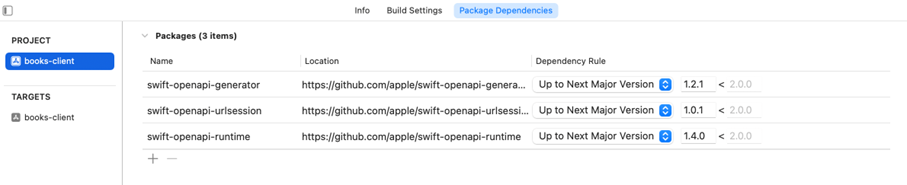
\includegraphics[scale=1.0]{../images/dependencies.png}
    \caption{Dependencies}
    
\end{figure}
\begin{figure}[htbp]
    \centering
    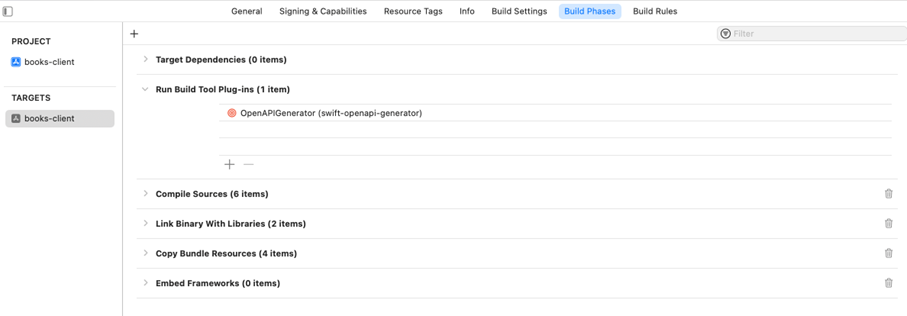
\includegraphics[scale=1.0]{../images/target.png}
    \caption{Run Build Tool Plug-ins}
    
\end{figure}



\subsubsection{Netwerklaag}
Nu wordt er de netwerklaag toevoeg aan het project. In deze netwerklaag wordt voor elk \textit{endpoint} een specifieke functie gecreëerd. Deze functies fungeren als de brug tussen de applicatie en de externe servers, waardoor communicatie mogelijk wordt via de API-\textit{endpoints}. Het bijzondere aan deze functies is dat er niet veel logica aan toegevoegd hoeft te worden, Veel van het proces wordt automatisch afgehandeld door de \textit{Client}. 
Hoewel de meeste van de logica automatisch wordt afgehandeld, er nog steeds aandacht moet worden besteed aan bepaalde aspecten, zoals \textit{error handling}. 

\begin{lstlisting}[caption=ApiService file]
import Foundation
import OpenAPIURLSession

class ApiService<C: APIProtocol> {
    let client : C
    
    init(client: C) {
        self.client = client
    }
    init() where C == Client {
        self.client = Client(
        serverURL: try! Servers.server1(),
        transport: URLSessionTransport()
        )
    }
    
    func getAllBooks() async -> [Components.Schemas.Book] {
        guard let response = try? await client.getAllBooks(Operations.getAllBooks.Input()) else {
            print("Error getting response")
            return []
        }
        
        switch response {
            case .ok(let okResponse):
            switch okResponse.body {
                case .json(let booksResponse):
                return booksResponse
            }
            case .undocumented(statusCode: let statusCode, _):
            print("Undocumented Error: \(statusCode)")
            return []
        }
    }
    
    func createBooks(book: Components.Schemas.Book) async -> Components.Schemas.Book {
        guard let response = try? await client.createBook(.init(body: .json(book))) else {
            print("Error getting response")
            return Components.Schemas.Book(id: "", title: "", author: "")
        }
        
        switch response {
            case .created(let okResponse):
            switch okResponse.body {
                case .json(let booksResponse):
                return booksResponse
            }
            case .undocumented(statusCode: let statusCode, _):
            print("Undocumented Error: \(statusCode)")
            return Components.Schemas.Book(id: "", title: "", author: "")
            case .badRequest(_):
            print("Bad Request")
            return Components.Schemas.Book(id: "", title: "", author: "")
        }
    }
    
    func updateBook(id: String, book: Components.Schemas.Book) async -> Components.Schemas.Book {
        guard let response = try? await client.updateBook(path: .init(id: id), body: .json(book)) else {
            print("Error getting response")
            return Components.Schemas.Book(id: "", title: "", author: "")
        }
        
        switch response {
            case .ok(let okResponse):
            switch okResponse.body {
                case .json(let booksResponse):
                return booksResponse
            }
            case .undocumented(statusCode: let statusCode, _):
            print("Undocumented Error: \(statusCode)")
            return Components.Schemas.Book(id: "", title: "", author: "")
            
        }
    }
    func getById(id: String) async -> Components.Schemas.Book {
        guard let response = try? await client.getById(path: .init(id: id)) else {
            print("Error getting response")
            return Components.Schemas.Book(id: "", title: "", author: "")
        }
        
        switch response {
            case .ok(let okResponse):
            switch okResponse.body {
                case .json(let booksResponse):
                return booksResponse
            }
            case .undocumented(statusCode: let statusCode, _):
            print("Undocumented Error: \(statusCode)")
            return Components.Schemas.Book(id: "", title: "", author: "")
            
            case .notFound(_):
            print("Not Found Error")
            return Components.Schemas.Book(id: "", title: "", author: "")
        }
    }
    
}

\end{lstlisting}

\subsubsection{Het creëren van de views}
Wanneer je netwerk laag gemaakt is, is zeer gemakkelijk om deze functies te gaan verwerken in je views. 

\begin{lstlisting}[caption=ApiService file]
struct ContentView: View {
    @State var BooksData = [Components.Schemas.Book]()
    @Environment(\.dismiss) var dismiss
    @State private var showAddBook = false
    var body: some View {
        VStack {
            NavigationView {
                List {
                    ForEach(BooksData, id: \.id) { book in
                        NavigationLink(destination: BookView(id: book.id)) {
                            Text("\(book.title) - \(book.author)")
                        }
                    }
                }.navigationTitle("Books")
                .toolbar {
                    Button {
                        showAddBook = true
                    }label: {
                        Label("add hotspot", systemImage: "plus.circle")
                    }
                }
            }
        }
        .onAppear{
            Task {
                BooksData = await ApiService().getAllBooks()
            }
        }.sheet(isPresented: $showAddBook, onDismiss: {
            Task {
                BooksData = await ApiService().getAllBooks()
            }
        }) {
            CreateBooks()
        }
    }
}

    
\end{lstlisting}
 \newpage
\section{Scenario 5: aanpasbaarheid van back-end}
Dit scenario wordt geïmplementeerd omdat het eventueel kan zijn dat er nog aanpassingen moeten gebeuren aan de back-end, nadat een \textit{client} is ontwikkeld. 
Specifiek in dit geval zou dat kunnen zijn om bijvoorbeeld extra gegevens toe te voegen aan een boek, namelijk beschrijving, \textit{genre}, … . 


\subsection{Technische doelstellingen}
Hoewel dit scenario niet bijzonder ingewikkeld is, is het cruciaal voor het onderzoeken van de flexibiliteit van een back-end die gebouwd is met de Swift OpenAPI-generator. Deze moet in staat zijn om veranderingen in het OpenAPI-document te accommoderen. Bijvoorbeeld, als er een nieuwe \textit{client} aan het systeem wordt toegevoegd, kunnen er wijzigingen in het OpenAPI-document nodig zijn om nieuwe eisen en functionaliteiten te weerspiegelen. Dit kan variëren van het toevoegen van nieuwe \textit{endpoints} tot het wijzigen van bestaande API-specificaties.

Het is belangrijk om te evalueren hoe flexibel en aanpasbaar de back-end is bij het omgaan met dergelijke veranderingen. Dit omvat de mogelijkheid om snel en efficiënt updates door te voeren in de back-end code en het waarborgen van consistentie en compatibiliteit tussen de OpenAPI-specificaties en de daadwerkelijke implementatie van de API-functionaliteit.

\subsubsection{Aanpasbaarheid back-end}
Het aanpassen van de back-end gaat zeer vlot, Er kunnen gemakkelijk wijzigingen gedaan worden aan het OpenAPI-document en kunnen gemakkelijk verwerkt worden in de \textit{handler}. Belangrijk om op te merken is dat de model en \textit{migration} niet mag vergeten aan te passen. Zo zijn er twee extra \textit{properties}  toegevoegd, namelijk \textit{genre} en beschrijving. 

\begin{lstlisting}[caption=openapi.yaml file]
components:
  schemas:
    Book:
      type: object
      properties:
        id:
          type: string
          format: uuid
          description: The ID of the book
        title:
          type: string
          description: The title of the book
        author:
          type: string
          description: The author of the book
        genre:
          type: string
          items:
            $ref: '#/components/schemas/Genre'
        description:
          type: string
      required:
        - id
        - title
        - author
        - genre
        - description
Genre:
  type: object
  properties:
    name:
      type: string
\end{lstlisting}

\begin{lstlisting}[caption=handler file]
struct Handler: APIProtocol {
    ……    
    func getAllBooks(_ input: Operations.getAllBooks.Input) async throws -> Operations.getAllBooks.Output {
        let books = try await Book.query(on: app.db).all()
        logger.info("successfull GET-request to database")
        
        var booksArray: Array<Components.Schemas.Book> = []
        books.forEach { book in
            booksArray.append(Components.Schemas.Book(id: "\(String(describing: book.id))", title: book.title, author: book.author, genre: book.genre.rawValue, description: book.description))
        }
        logger.info("Converted books of database to return object")
        return .ok(.init(body: .json(booksArray)))
    }
    
    func getById(_ input: Operations.getById.Input) async throws -> Operations.getById.Output {
        let id = UUID(uuidString: input.path.id)
        guard let book = try await Book.find(id, on: app.db) else {
            logger.debug("Can't find Book in database!")
            throw Abort(.notFound)
        }
        
        return .ok(.init(body: .json(Components.Schemas.Book(id: "\(String(describing: book.id))", title: book.title, author: book.author, genre: book.genre.rawValue, description: book.description))))
        
    }
    
    
    func createBook(_ input: Operations.createBook.Input) async throws -> Operations.createBook.Output {
        guard case .json(let bookInput) = input.body else {
            logger.debug("Something went wrong with the Input.body")
            fatalError()
        }
        
        let id = UUID(uuidString: bookInput.id)
        
        //validations of book
        if (bookInput.title.isEmpty || bookInput.author.isEmpty) {
            throw Abort(.badRequest, reason: "Invalid title or author")
        }
        
        var book = Book(id: id, title: bookInput.title, author: bookInput.author, genre: Genre(rawValue: bookInput.genre) ?? Genre.Roman, description: bookInput.description)
        try await book.save(on: app.db)
        
        let bookapi: Components.Schemas.Book
        switch input.body {
            case .json(let json): bookapi = json
            case .none:
            bookapi = .init(id: "", title: "", author: "", genre: "", description: "")
            break
        }
        
        return .created(.init(body: .json(bookapi)))
    }
    
    func updateBook(_ input: Operations.updateBook.Input) async throws -> Operations.updateBook.Output {
        guard case .json(let bookInput) = input.body else {
            logger.debug("Something went wrong with the Input.body")
            fatalError()
        }
        //validations of book
        if (bookInput.title.isEmpty || bookInput.author.isEmpty) {
            throw Abort(.badRequest, reason: "Invalid title or author")
        }
        
        let id = UUID(uuidString: bookInput.id)
        guard let bookDb = try await Book.find(id, on: app.db) else {
            throw Abort(.notFound)
        }
        bookDb.id = UUID(uuidString: bookInput.id)
        bookDb.title = bookInput.title
        bookDb.author = bookInput.author
        bookDb.genre = Genre(rawValue: bookInput.genre) ?? Genre.Roman
        bookDb.description = bookInput.description
        
        try await bookDb.update(on: app.db)
        
        let updatedBook: Components.Schemas.Book
        switch input.body {
            case .json(let json): updatedBook = json
            case .none:
            updatedBook = .init(id: "", title: "", author: "", genre:"", description: "")
            break
        }
        return .ok(.init(body: .json(updatedBook)))
    }
    ………
    
}

\end{lstlisting}

\subsubsection{Aanpasbaarheid front-end}
Het aanpassen van de front-end gaat ook zeer vlot.Belangrijk om op te merken is dat het OpenAPI-document overeenkomt met dat in de back-end. Hierna moet de netwerklaag nog aangepast worden naar de \textit{endpoints} of nieuwe gegevens van de \textit{components}, dit is enkel de \textit{error handling}. En dan kan gestart worden met het verwerken van de nieuwe gegevens in de UI.

\begin{lstlisting}[caption=ApiService file]
class ApiService<C: APIProtocol> {
    let client : C
    
    init(client: C) {
        self.client = client
    }
    init() where C == Client {
        self.client = Client(
        serverURL: try! Servers.server1(),
        transport: URLSessionTransport()
        )
    }
    
    func getAllBooks() async -> [Components.Schemas.Book] {
        guard let response = try? await client.getAllBooks(Operations.getAllBooks.Input()) else {
            print("Error getting response")
            return []
        }
        
        switch response {
            case .ok(let okResponse):
            switch okResponse.body {
                case .json(let booksResponse):
                return booksResponse
            }
            case .undocumented(statusCode: let statusCode, _):
            print("Undocumented Error: \(statusCode)")
            return []
        }
    }
    
    func createBooks(book: Components.Schemas.Book) async -> Components.Schemas.Book {
        guard let response = try? await client.createBook(.init(body: .json(book))) else {
            print("Error getting response")
            return Components.Schemas.Book(id: "", title: "", author: "", genre: "", description: "")
        }
        
        switch response {
            case .created(let okResponse):
            switch okResponse.body {
                case .json(let booksResponse):
                return booksResponse
            }
            case .undocumented(statusCode: let statusCode, _):
            print("Undocumented Error: \(statusCode)")
            return Components.Schemas.Book(id: "", title: "", author: "", genre: "", description: "")
            case .badRequest(_):
            print("Bad Request")
            return Components.Schemas.Book(id: "", title: "", author: "", genre: "", description: "")
        }
    }
    
    func updateBook(id: String, book: Components.Schemas.Book) async -> Components.Schemas.Book {
        guard let response = try? await client.updateBook(path: .init(id: id), body: .json(book)) else {
            print("Error getting response")
            return Components.Schemas.Book(id: "", title: "", author: "", genre: "", description: "")
        }
        
        switch response {
            case .ok(let okResponse):
            switch okResponse.body {
                case .json(let booksResponse):
                return booksResponse
            }
            case .undocumented(statusCode: let statusCode, _):
            print("Undocumented Error: \(statusCode)")
            return Components.Schemas.Book(id: "", title: "", author: "", genre: "", description: "")
            
        }
    }
    func getById(id: String) async -> Components.Schemas.Book {
        guard let response = try? await client.getById(path: .init(id: id)) else {
            print("Error getting response")
            return Components.Schemas.Book(id: "", title: "", author: "", genre: "", description: "")
        }
        
        switch response {
            case .ok(let okResponse):
            switch okResponse.body {
                case .json(let booksResponse):
                return booksResponse
            }
            case .undocumented(statusCode: let statusCode, _):
            print("Undocumented Error: \(statusCode)")
            return Components.Schemas.Book(id: "", title: "", author: "", genre: "", description: "")
            
            case .notFound(_):
            print("Not Found Error")
            return Components.Schemas.Book(id: "", title: "", author: "", genre: "", description: "")        }
    }
    
}

\end{lstlisting}

% Voeg hier je eigen hoofdstukken toe die de ``corpus'' van je bachelorproef
% vormen. De structuur en titels hangen af van je eigen onderzoek. Je kan bv.
% elke fase in je onderzoek in een apart hoofdstuk bespreken.

%\input{...}
%\input{...}
%...

%%=============================================================================
%% Conclusie
%%=============================================================================

\chapter{Conclusie}%
\label{ch:conclusie}

In dit onderzoek wordt er een antwoord gegeven op de onderzoeksvraag : “In hoeverre is de \textit{Swift OpenAPI Generator} in staat om snel een werkend prototype te genereren dat zowel geschikt is voor demonstratie- doeleinden als kan evolueren tot een productieklare back-end zonder dat een herimplementatie nodig is ”. Om een antwoord te geven op deze vraag werd de \textit{Swift OpenAPI Generator} aan de hand van scenario’s uitgebreid getest. 
\\ \\
Uit dit onderzoek komen diverse bevindingen naar voren. Ten eerste wordt duidelijk dat het integreren van een database op een relatief eenvoudige en doeltreffende manier kan worden gerealiseerd. Dit werd gerealiseerd door \textit{migrations} en models toe te voegen aan het project. Gedurende het volledige ontwikkelproces van de back-end is het mogelijk om flexibel aanpassingen door te voeren aan het OpenAPI-document. Dit geeft ontwikkelaars de ruimte om te experimenteren en aanpassingen te maken waar nodig. 
\\ \\
Daarnaast is het mogelijk om diverse facetten van back-end logica toe te voegen. Deze facetten omvatten belangrijke elementen zoals \textit{logging}, \textit{metrics} en validatie. Interessant is dat \textit{logging} zowel op de standaardmethode als via een meer complexe \textit{middleware} kan worden geïmplementeerd. \textit{Metrics} kunnen eveneens worden toegevoegd met behulp van \textit{middleware}. Validatie kan op een iets minder efficiënte manier worden toegevoegd. 
\\ \\
Om validatie toe te voegen werd aanvankelijk geprobeerd om models te gebruiken voor het valideren van gegevens, maar al snel bleek dit niet haalbaar vanwege de discrepanties tussen de gebruikte validatiemethoden en de \textit{Swift OpenAPI Generator}. Een alternatieve benadering, gebaseerd op het format zoals gespecificeerd in het OpenAPI-document, leek veelbelovend maar werkte niet goed met de \textit{generator}. 
Uiteindelijk werd gekozen voor een pragmatische aanpak waarbij handmatige validatie werd uitgevoerd in de \textit{handler} voordat gegevens werden opgeslagen. Hoewel dit effectief bleek te zijn en voldeed het aan de validatiebehoeften, is dit zeer arbeidsintensief en zou het handiger zijn als je de validatie zou kunnen toevoegen aan het OpenAPI document. 
\\ \\
Een andere cruciale bevinding die uit het gedetailleerde onderzoek naar voren kwam, betreft de kwestie van authentificatie. Hier zijn nog enkele uitdagingen die aandacht vereisen en waarvoor verdere verbeteringen en innovaties absoluut noodzakelijk zijn om de efficiëntie en veiligheid van het systeem te waarborgen.
\\ \\
Tot slot, maar zeker niet onbelangrijk, is het vermeldenswaardig dat de back-end, die zorgvuldig is ontworpen en gemaakt met behulp van de \textit{Swift OpenAPI Generator}, naadloos kan worden geïntegreerd in een \textit{client}applicatie. Dit is een belangrijke stap die kan worden bereikt door simpelweg de benodigde \textit{dependencies} toe te voegen en een geschikte netwerklaag te implementeren. Deze belangrijke bevindingen bieden waardevolle inzichten en vormen een solide basis voor verdere ontwikkeling en optimalisatie van de applicatiearchitectuur in de toekomst.
\\ \\
Hoewel de \textit{Swift OpenAPI Generator} over het algemeen geschikt is voor het genereren van een back-end, wordt de complexiteit ervan duidelijk wanneer men meer geavanceerde functies zoals authentificatie wil toevoegen. In mijn ervaring is de \textit{Swift OpenAPI Generator} een waardevol hulpmiddel voor educatieve doeleinden, waarbij het studenten in staat stelt om gemakkelijk een back-end op te stellen, zonder echte back-end kennis. Echter, bij het ontwikkelen van een complexere back-end, zijn aanpassingen aan de generator noodzakelijk om aan de vereisten te voldoen.

%---------- Bijlagen -----------------------------------------------------------

\appendix

\chapter{Onderzoeksvoorstel}

Het onderwerp van deze bachelorproef is gebaseerd op een onderzoeksvoorstel dat vooraf werd beoordeeld door de promotor. Dat voorstel is opgenomen in deze bijlage.

%% TODO: 
%\section*{Samenvatting}

% Kopieer en plak hier de samenvatting (abstract) van je onderzoeksvoorstel.

% Verwijzing naar het bestand met de inhoud van het onderzoeksvoorstel
%---------- Inleiding ---------------------------------------------------------

\section{Introductie}%
\label{sec:introductie}
In het snel evoluerende domein van software-ontwikkeling wordt de behoefte aan flexibele en efficiënte tools om het ontwikkelingsproces te versnellen en te vereenvoudigen steeds belangrijker. Bij de introductie van de Swift OpenAPI Generator in juni, dacht men dat deze tool hiervoor een veelbelovende oplossing zou kunnen zijn. Dit onderzoek richt zich op de mogelijkheden van de Swift OpenAPI Generator, met specifieke focus op het vermogen om een werkend prototype te genereren en ook op hoe gemakkelijk het kan evolueren naar een productieklare back-end zonder een volledige herimplementatie. 

De doelstelling van dit onderzoek bestaat uit twee delen. Enderzijds richt het zich op het beoordelen van de capaciteiten van de Swift OpenAPI Generator. Anderzijds bestudeert het de haalbaarheid en efficiëntie van het evolueren van een prototype naar een productieklare back-end. 

Het concrete eindresultaat van dit onderzoek bestaat niet alleen uit een uitgeschreven scriptie, maar ook uit een tastbaar bewijs van de Swift OpenAPI Generator in actie. Het zal als een succesvolle bachelorproef beschouwd worden wanneer op een gemakkelijke manier een back-end kan gegenereerd worden die we als een productieklare back-end kunnen zien zonder dat er veel aanpassingen nog nodig zijn. Een rapport met aanbevelingen voor verdere optimalisatie en implementatie zou het sluitstuk kunnen vormen, waarbij het geheel als succesvol wordt beschouwd wanneer de Swift OpenAPI Generator daadwerkelijk bijdraagt aan het versnellen en vereenvoudigen van het ontwikkelingsproces.  

%---------- Stand van zaken ---------------------------------------------------

\section{Literatuurstudie}%
\label{sec:literatuurstudie}
De Swift OpenAPI Generator is een swift plugin, die code kan genereren die nodig is om API-oproepen te doen of API servers te implementeren. Het genereert de code aan de hand van de openAPI documenten. Dit zorgt ervoor dat Swift-ontwikkelaars snel en efficiënt clientcode kunnen genereren voor het gebruik van RESTfull API’s. Om de swift OpenAPI Generator te gebruiken moet je twee plugins toevoegen, de swift-openapi-generator en de swift-openapi-runtime. De eerste plugin genereert code tijdens build-time en de tweede plugin bevat protocol definities die worden gebruikt door de gegenereerde code en extensiebibliotheken.Hierna moet je nog 2 bestanden toevoegen aan uw project namelijk de openapi.yaml, beschrijft uw API, de openapi-generator-config.yaml is een configuratiebestand voor de plug-in die bepaalt of client- of servercode moet worden gegenereerd. Met zijn intuïtieve interface, uitgebreide functies en sterke community-ondersteuning is het een essentiële troef voor elke Swift-ontwikkelaar die met API's werkt  \autocite{Dvorsky2023} . 

De openAPI document is een open standaard voor het definiëren van HTTP APIs, meestal gedocumenteerd in YAML of JSON. OpenAPI-documenten zijn een essentieel hulpmiddel om consistentie en kwaliteit te waarborgen tijdens de ontwikkeling, doordat ze verschillende doeleinden dienen. De openAPI-documenten worden opgesteld volgens de OpenAPI-specificaties (OAS) en deze specificaties zorgen voor duidelijke, leesbare beschrijving van HTTP API’s voor zowel mensen als machines die het mogelijk maken een service te begrijpen zonder dat er veel kennis nodig is om met de service te communiceren \autocite{Miller2020}. 

Hoewel OpenAPI en Swagger verwant zijn, zijn ze niet identiek. OpenAPI vertegenwoordigt de evolutie van de Swagger 2.0-specificatie, die een nieuwe naam kreeg na de overname door SmartBear Software en de donatie aan het OpenAPI Initiative \autocite{2023}. OpenAPI is de specificatie die wordt gebruikt om RESTfull API's te definiëren. Swagger omvat een reeks tools die worden gebruikt om OpenAPI specification te implementeren. Swagger bevat ook een breed scala aan API-ontwerp-, documentatie-, test-, beheer- en monitoring-oplossingen die het voor ontwikkelaars gemakkelijker maken om de openAPI specificaties te implementeren \autocite{ Pinkham2017}. 

Een van de best practices om een API te ontwikkelen is om een API te creëren volgens de design principes van REST. Representational State Transfer is ontworpen om als richtlijn te dienen voor het beheren van communicatie binnen complexe netwerken zoals het internet. API’s die gebruik maken van REST worden REST API’s of RESTfull API’s genoemd. De principes van REST-architectuurstijl omvatten een uniforme interface, statelessness, een gelaagd systeem, cachebaarheid en code on demand. Door deze principes biedt Rest API verschillende voordelen, namelijk schaalbaarheid, flexibiliteit en onafhankelijkheid van specifieke technologieën. Dit betekent dat zowel client- als server-applicaties in verschillende programmeertalen kunnen worden geschreven zonder dat dit invloed heeft op het API-ontwerp \autocite{2020}. 

Het creëren van back-end in Swift wordt voornamelijk gedaan via Vapor. Het is een open-source web framework die geschreven is in Swift en is een krachtig framework voor het schrijven van web- en API-services \autocite{Nelson}. Vapor profiteert ook van het concurrency-model van Swift, deze maakt deelbare, veranderlijke status- en datarace-veiligheid mogelijk, waardoor een betrouwbaar en efficiënt framework kan worden aangeboden. Bovendien heeft Swift de laagste geheugen-voetafdruk van native gecompileerde binaire bestanden in Linux, waardoor Vapor een lichtgewicht en efficiënte keuze is. Het heeft een kleine leercurve voor native app-ontwikkelaars, waardoor het een go-to-oplossing is voor de ontwikkeling van API-services \autocite{Pant2023}.
% Voor literatuurverwijzingen zijn er twee belangrijke commando's:
% \autocite{KEY} => (Auteur, jaartal) Gebruik dit als de naam van de auteur
%   geen onderdeel is van de zin.
% \textcite{KEY} => Auteur (jaartal)  Gebruik dit als de auteursnaam wel een
%   functie heeft in de zin (bv. ``Uit onderzoek door Doll & Hill (1954) bleek
%   ...'')



%---------- Methodologie ------------------------------------------------------
\section{Methodologie}%
\label{sec:methodologie}

Voor het onderzoek naar de mogelijkheden van de Swift OpenAPI Generator is er een plan van aanpak. Dit plan van aanpak is opgedeeld in verschillende fases. 

In de eerste fase is het doel om een diepgaande kennis te verwerven over het onderwerp. Deze fase wordt opgedeeld in 3 deelfases. Als eerste richt men zich op de OpenAPI specificaties, omdat de Swift OpenAPI Generator sterk afhankelijk is van deze specificaties. Dit wordt gedaan om inzicht te krijgen over hoe OpenAPI wordt gebruikt in andere contexten om zicht te krijgen op de generieke bruikbaarheid van de OpenAPI specificaties. Naast het begrijpen van de OpenAPI specificaties, is het belangrijk dat er gekeken wordt naar de best practices en trends van de API-ontwikkeling en hoe back-ends doorgaans ontwikkeld en geoptimaliseerd worden. Hierna is van groot belang dat er gefocust wordt op het gebruik van Swift in Backend-ontwikkeling. 

Na deze eerste fase zullen er duidelijke doelstellingen worden bepaald voor het verder verloop van het onderzoek. Aan de hand van de literatuurstudie zullen deze doelstellingen worden vastgelegd om een duidelijk beeld te krijgen van wat de Swift OpenAPI Generator allemaal moet kunnen, namelijk is de Swift OpenAPI generator instaat om authentificatie of validatie toe te passen en API calls te beperken tot een specifieke rol. 

In de derde fase zullen er twee deelfases uitgewerkt worden. In de eerste deelfase zullen er mogelijk scenario's worden gecreëerd om de Swift OpenAPI-generator te testen. Er zullen vijf verschillende scenario's worden uitgewerkt, waarbij elke keer een iets complexere API nodig zal zijn. Hierbij zullen de OpenAPI-specificaties en de literatuurstudie worden gebruikt om de mogelijke scenario's uit te werken. Nadat deze scenario’s zijn uitgeschreven kan er werk gemaakt worden van de tweede deelfase. In de volgende fase zal een Swift UI uitgewerkt worden waarbij je gemakkelijk kan zien hoe deze API’s werken. Deze Swift UI zal gebruikt worden om na te gaan of het mogelijk is om een snelwerkend prototype te creëren. 

In de volgende fase zullen alle mogelijke scenario’s worden uitgewerkt met de Swift OpenAPI Generator. Ook zullen ze getest worden met de Swift UI die gecreëerd is in de voorgaande fase. Deze fase wordt gedaan om te weten te komen hoe gemakkelijk het is om een werkend prototype te genereren. 

Na deze fase zullen de verzamelde gegevens geanalyseerd worden om inzicht te krijgen in de prestaties van de Swift OpenAPI Generator. Ook zullen de gegevens met elkaar worden vergeleken en zal het meest effectieve scenario worden geïdentificeerd aan de hand van de vooraf bepaalde doelstellingen. Ook zullen de eventuele beperkingen van de Swift OpenAPI Generator worden geïdentificeerd.

Als laatste zal er een conclusie worden getrokken uit het onderzoek en een antwoord worden geformuleerd op de onderzoeksvraag op basis van de verkregen resultaten. Ook zal er een aanbeveling worden geschreven voor het gebruik van de Swift OpenAPI generator. 



%---------- Verwachte resultaten ----------------------------------------------
\section{Verwacht resultaat, conclusie}%
\label{sec:verwachte_resultaten}

Aan de hand van mijn literatuurstudie kan er afgeleid worden dat de Swift OpenAPI generator goed zal werken bij gemakkelijkere API’s, maar minder goed bij complexere API’s. Bij voorgaande tools die code genereren is het vaak zo dat er nog veel zaken moeten aangepast worden, maar wanneer je dit opnieuw laat genereren ben je je aanpassingen weer kwijt en moet je weer opnieuw beginnen. Zelf hoop ik dat ik deze verwachtingen kan weerleggen, zou het een zeer nuttig instrument kunnen zijn voor het ontwikkelen van een back-end. Dit zou ervoor zorgen dat de developers meer tijd kunnen besteden aan de apps interface. 

%%---------- Andere bijlagen --------------------------------------------------
% TODO: Voeg hier eventuele andere bijlagen toe. Bv. als je deze BP voor de
% tweede keer indient, een overzicht van de verbeteringen t.o.v. het origineel.
%\input{...}

%%---------- Backmatter, referentielijst ---------------------------------------

\backmatter{}

\setlength\bibitemsep{2pt} %% Add Some space between the bibliograpy entries
\printbibliography[heading=bibintoc]

\end{document}
